\documentclass[11pt, oneside]{article} 
\usepackage{geometry}                		
\geometry{letterpaper}                   		
\usepackage{graphicx}
\usepackage{graphics}
\usepackage{hyperref}
\usepackage{fancybox}
\usepackage[centertags]{amsmath}
\usepackage{amssymb}
\usepackage{amsthm}			
\usepackage{natbib}				
\usepackage{fullpage}
\usepackage{placeins}
\usepackage{setspace}
\usepackage{lineno}
%\usepackage{figcaps}
\usepackage[tablesfirst,nolists]{endfloat}
\usepackage{authblk}
\usepackage{csvsimple}


\DeclareRobustCommand{\firstsecond}[2]{#1}

\newcommand{\mb}{\mathbf}
\newcommand{\bs}{\boldsymbol}
\newcommand{\wt}{\widetilde}
\newcommand{\s}{^{(s)}}

\title{Supplemental Methods}

\author[1]{}
\author[2]{}
\author[3]{}

\date{\today}

\begin{document}
\maketitle

\doublespacing

\section {Data overview}
This document briefly describes the data cleaning, subsetting, and aggregation methods specific to each dataset.
%Table \ref{metadata} shows metadata on the datasets included in the meta-analysis.
We plot species accumulation curves, spatio-temporal variation in the number of taxa observed, the spatio-temporal sampling effort, and the number of taxa shared by each pairwise combination of plots within the study.
%We also identify any potential issues with the data.
We visually evaluated the species accumulation curves and temporal patterns in species abundances. % to screen for changes in sampling methods or data recording methods over the course of the study that could affect results.
A sudden jump in the cumulative number of taxa, for example, could indicate that taxa were recorded to a finer resolution (not that more taxa appeared  at the site).  
A species accumulation curve that does not level off could indicate a community undergoing rapid succession, invasion, or environmental change. 

For each dataset, we evaluated whether all sites were observed with equal effort in all years of study and we document any years, sites, sampling occasions,  or species that were droppped from the dataset prior to analysis. 
We also document the method used to aggregate the data to an annual value for each species at each site.
We visually evaluated the species accumulation curves and temporal patters in species abundances to screen for changes in sampling methods or data recording methods over the course of the study that could affect results.
For example, a sudden jump in the number of taxa in a given year could indicate that taxa were recorded to a finer resolution (not that more taxa were actually present at the site).  
We also checked to be sure an abundance of zero was recorded for each absence (i.e. we made sure zeros were filled in for site-years in which a species was not observed).
We removed species codes that obviously represent`unknown' species.
{\bf Do we use cutoff criteria to remove rare species prior to analysis? 
If so, we  should probably include that code in formatting script for each site so that the Supplemental figures and L3 data product we publish match the data used in analysis.}
We also include a table of datasets that were considered, and that we prepared into the L3 format, but ultimately were not included in the analysis (Table \ref{not_used}).


\begin{table}[h!]
\scriptsize
   \centering
     \caption{Metadata on the data sets included in the meta-analysis. This table is automatically generated directly from the datasets in the L3 folder.} 

\csvautotabular{metadata_table.csv}
   \label{metadata} 
\end{table}


%%%%%%%%%%%%%%%%%%%%%
\section {Marine datasets}


\subsection {csun.usvi-coral}
Data were downloaded from \url{http://mcrlter.msi.ucsb.edu/cgi-bin/showCSUNDataset.cgi?docid=knb-csun-usvi.101.4}.
Need more metadata for this dataset.
Margaret is helping.
Data are in Figure \ref{usvi-coral}.

\begin{figure}[h!]
\centering
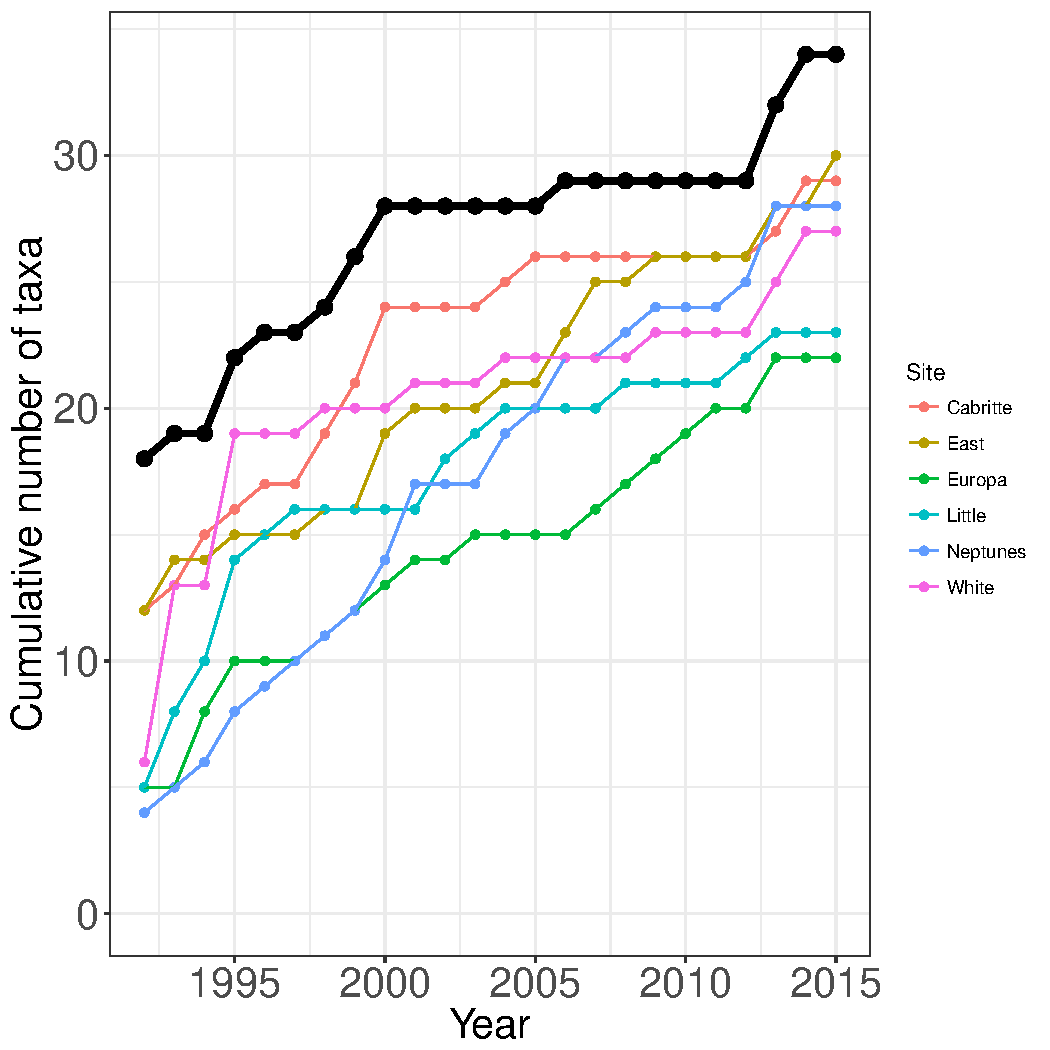
\includegraphics[scale = 0.4]{usvi-coral-castorani_species_accumulation_curve.pdf}
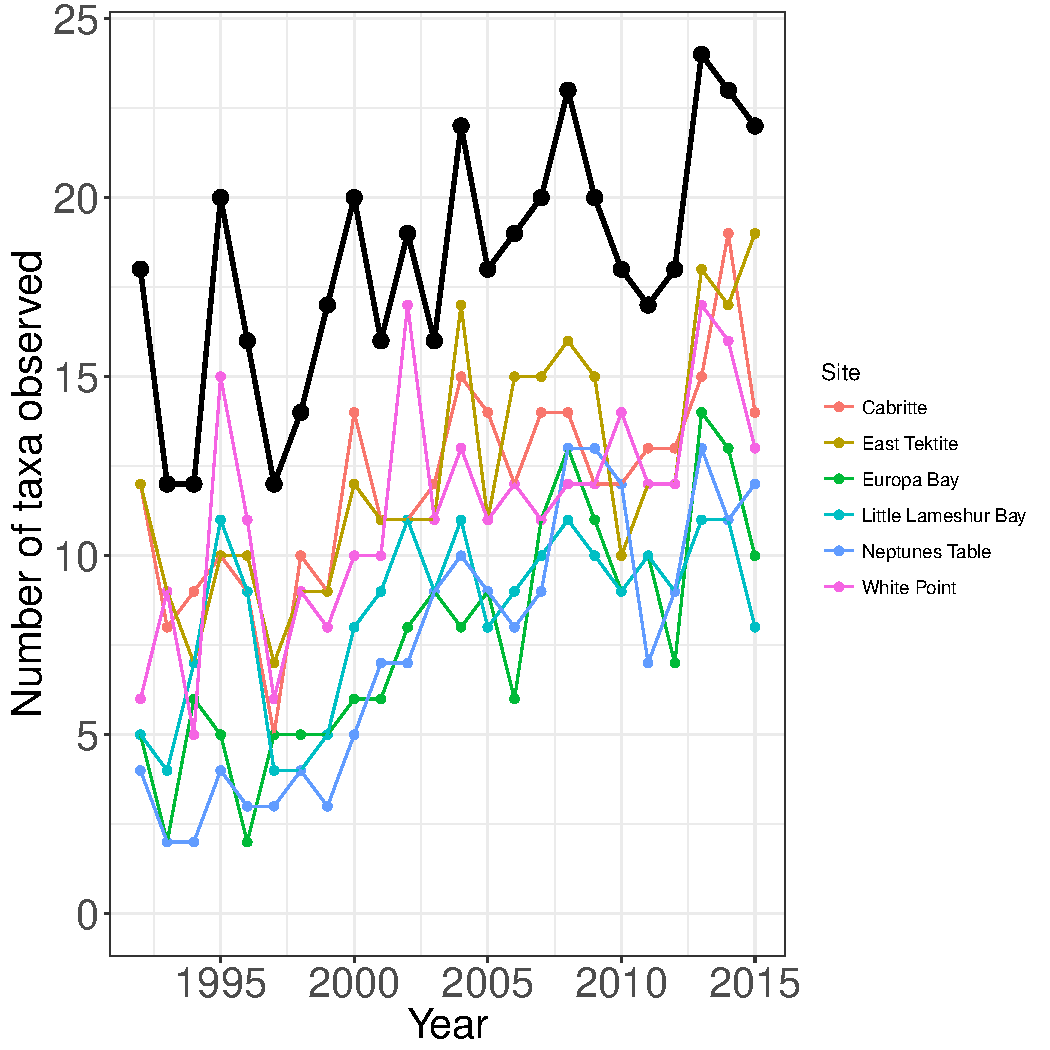
\includegraphics[scale = 0.4]{usvi-coral-castorani_num_taxa_over_time.pdf}
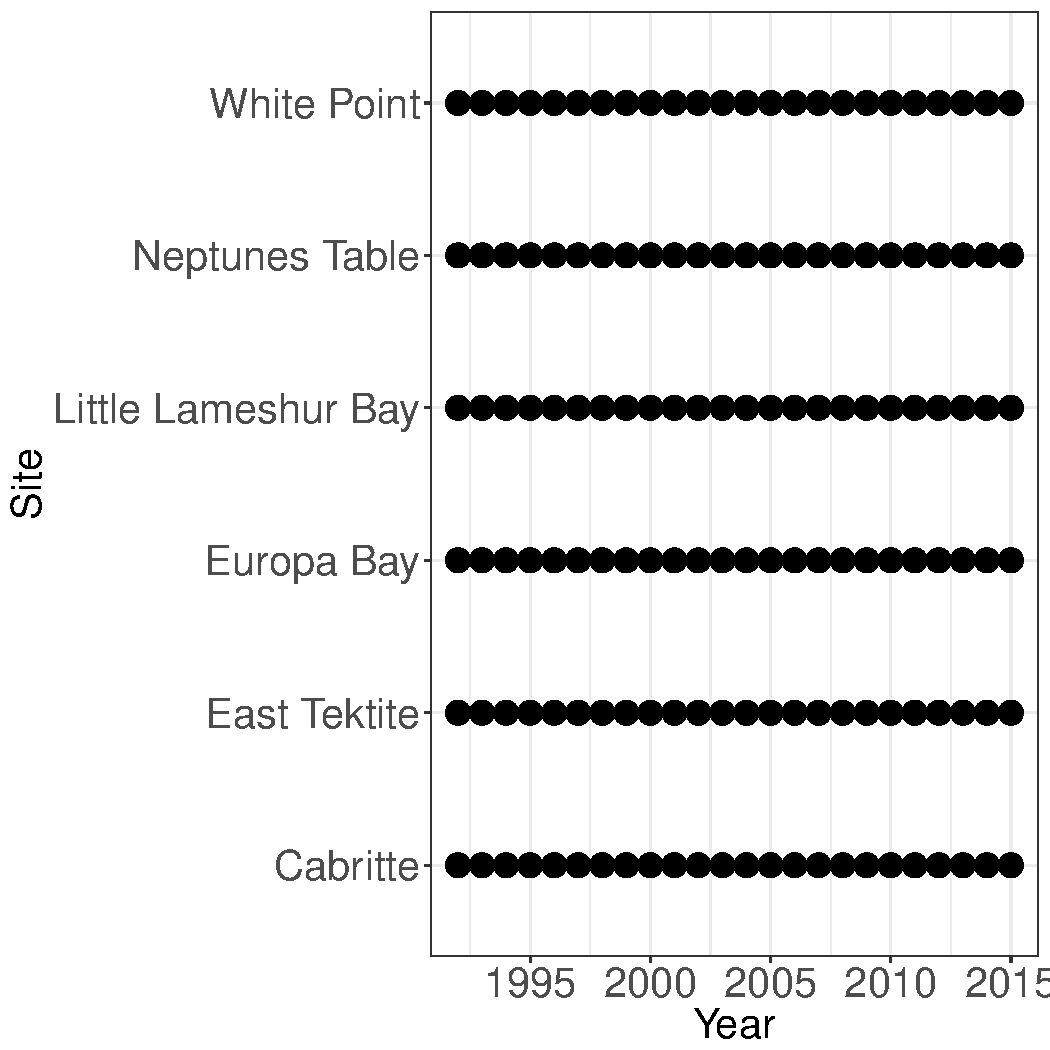
\includegraphics[scale = 0.4]{usvi-coral-castorani_spatiotemporal_sampling_effort.pdf}
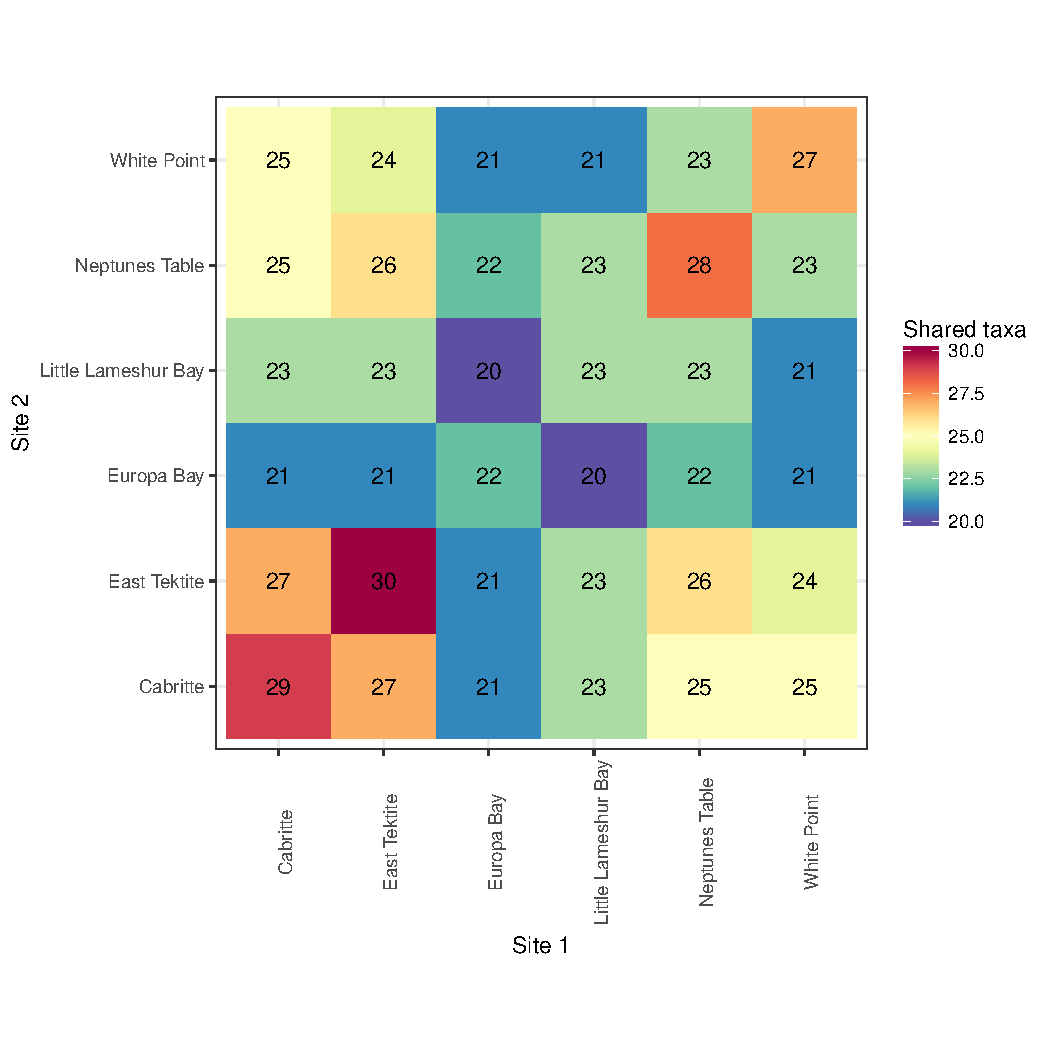
\includegraphics[scale = 0.4]{usvi-coral-castorani_spp_shared.pdf}
\caption{{\bf USVI-corals:} Species accumulation curves (top left),  annual richness (top right), sampling effort (bottom left), and number of shared species (bottom right)  for 34 coral taxa observed at 6 plots on St. John, US Virgin Islands (1990-2005). The black lines represent total site-level values across all plots.}
\label{usvi-coral}
\end{figure}

\subsection {sbc-survey-algae}
{\bf Waiting for updated data to be archived on EDI.}
Two of the eleven sites were initiated in the third year of study.
I think we should remove the two sites.
Data are shown in Figure \ref{sbc-algae}
\begin{figure}[h!]
\centering
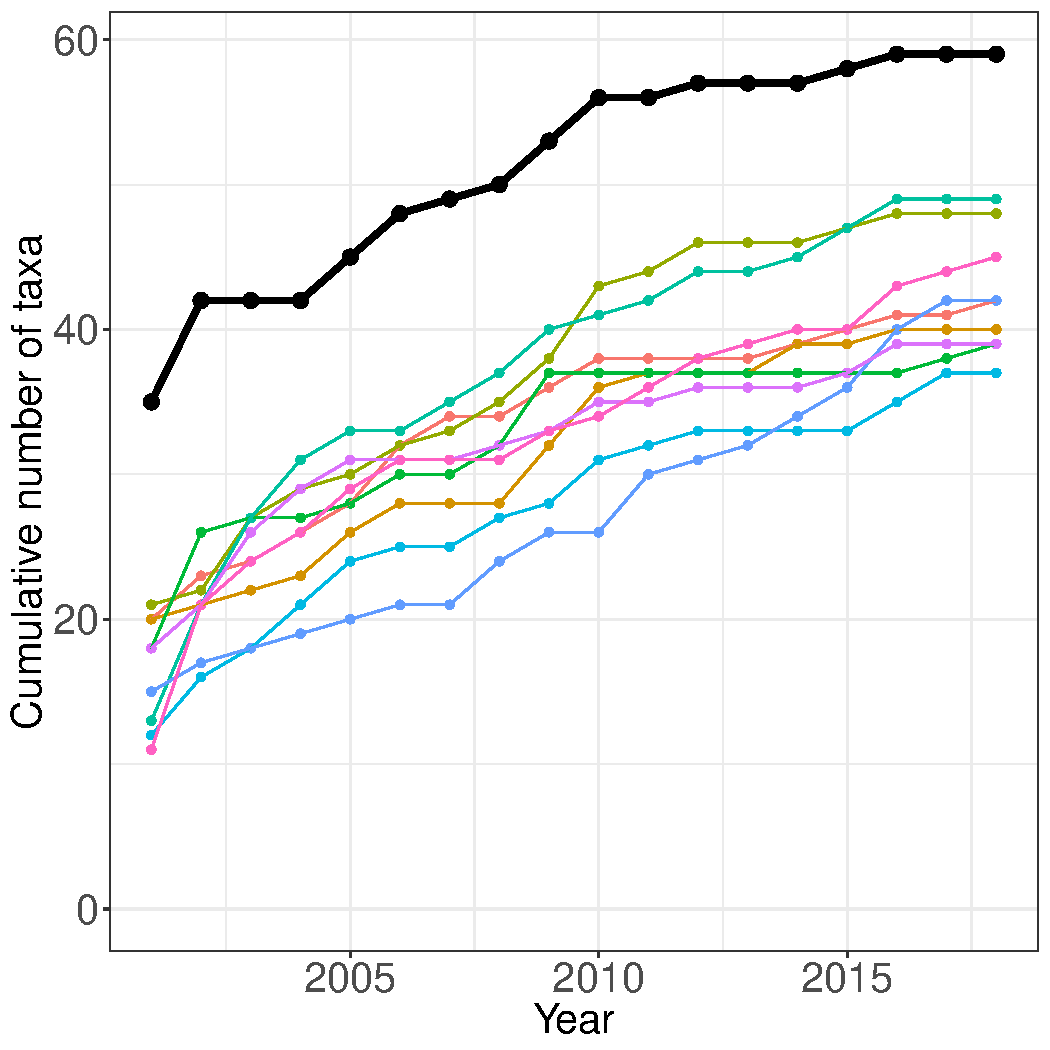
\includegraphics[scale = 0.4]{sbc-algae-castorani_species_accumulation_curve.pdf}
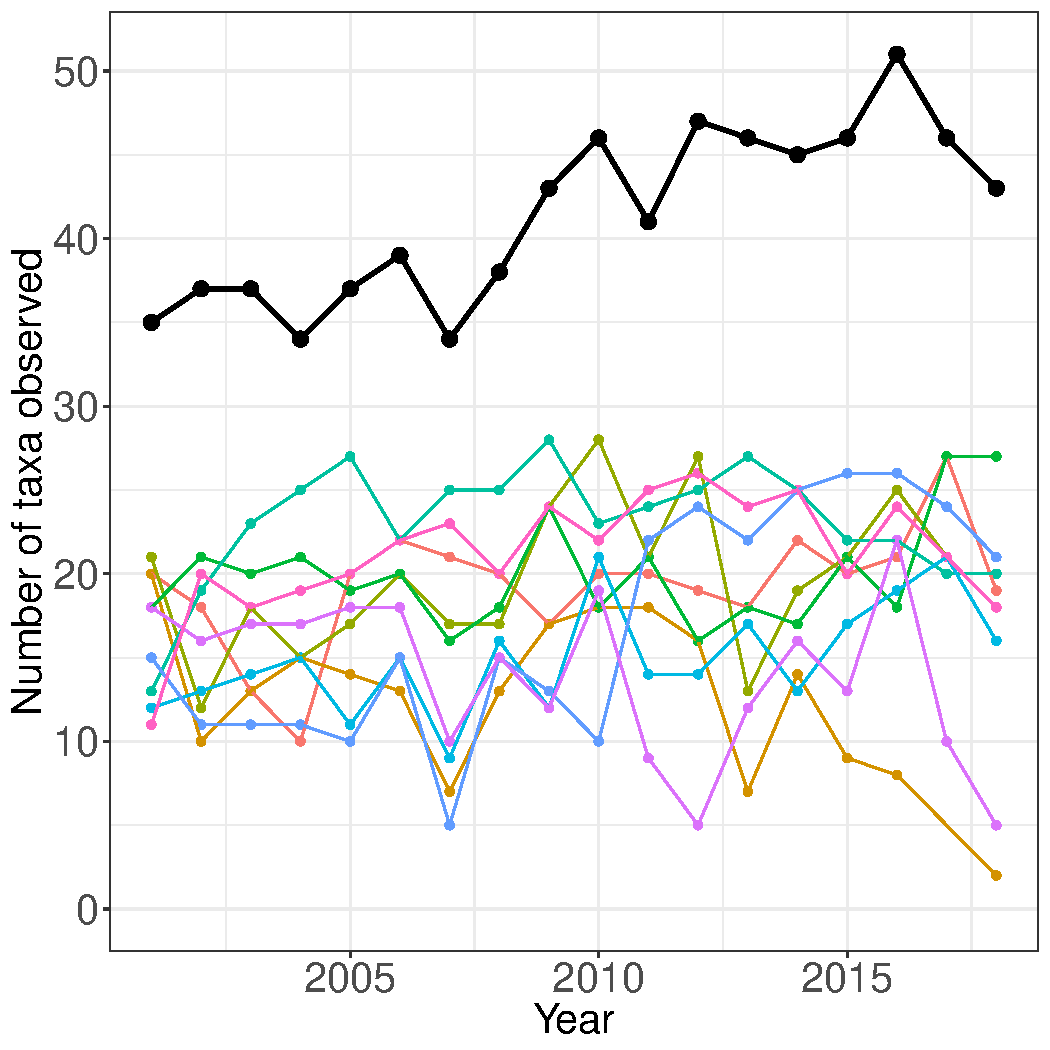
\includegraphics[scale = 0.4]{sbc-algae-castorani_num_taxa_over_time.pdf}
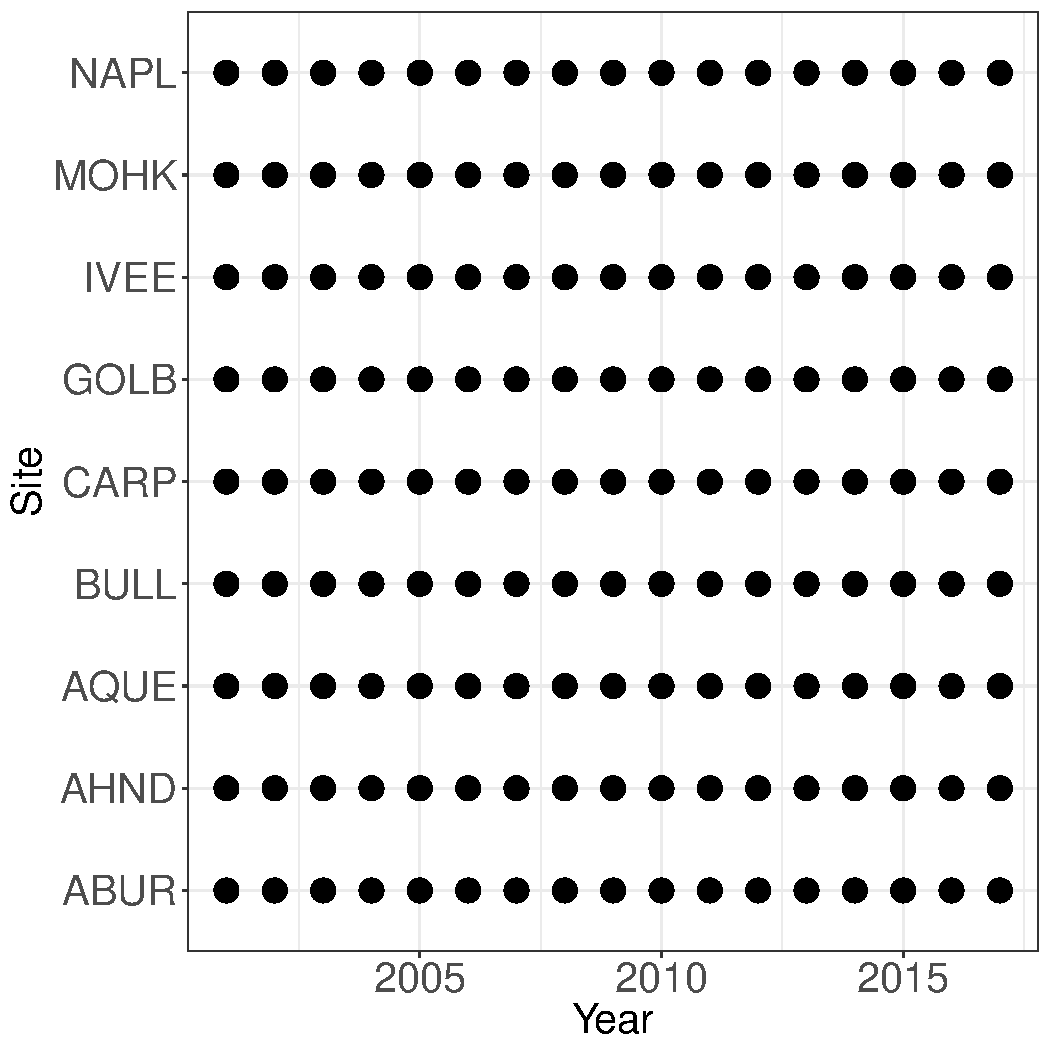
\includegraphics[scale = 0.4]{sbc-algae-castorani_spatiotemporal_sampling_effort.pdf}

\caption{{\bf SBC-algae:} Species accumulation curves (top left),  annual richness (top right), and sampling effort (bottom)  for 62 algae taxa observed at 11 plots in the Santa Barbara Channel LTER (2001-2016). The black lines represent total site-level values across all plots.}
\label{sbc-algae}
\end{figure}

\subsection {sbc-survey-sessile-inverts}
{\bf Waiting for updated data to be archived on EDI.}
Two of the eleven sites were initiated in the third year of study.
I think we should remove the two sites.
Data are shown in Figure \ref{sbc-sessileInverts}
\begin{figure}[h!]
\centering
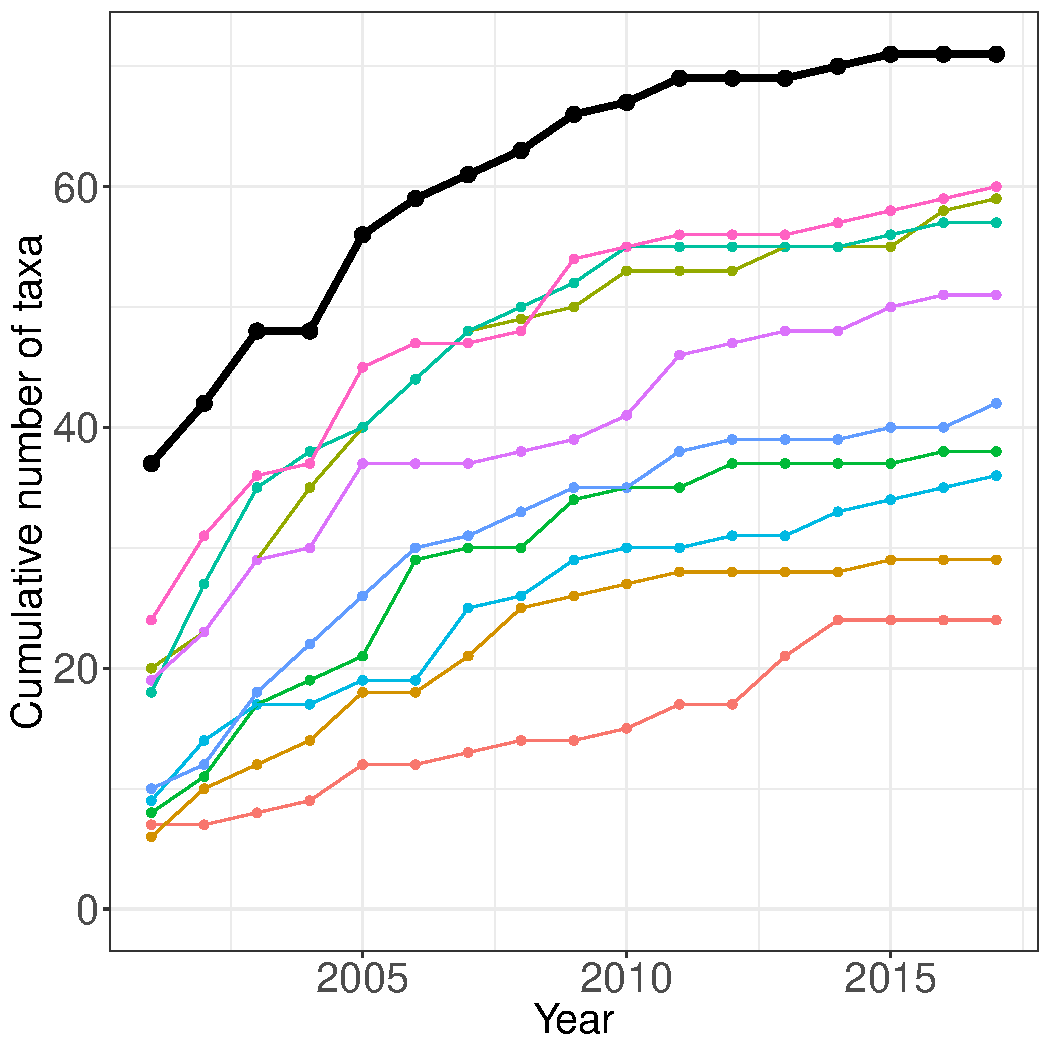
\includegraphics[scale = 0.4]{sbc-sessileInverts-castorani_species_accumulation_curve.pdf}
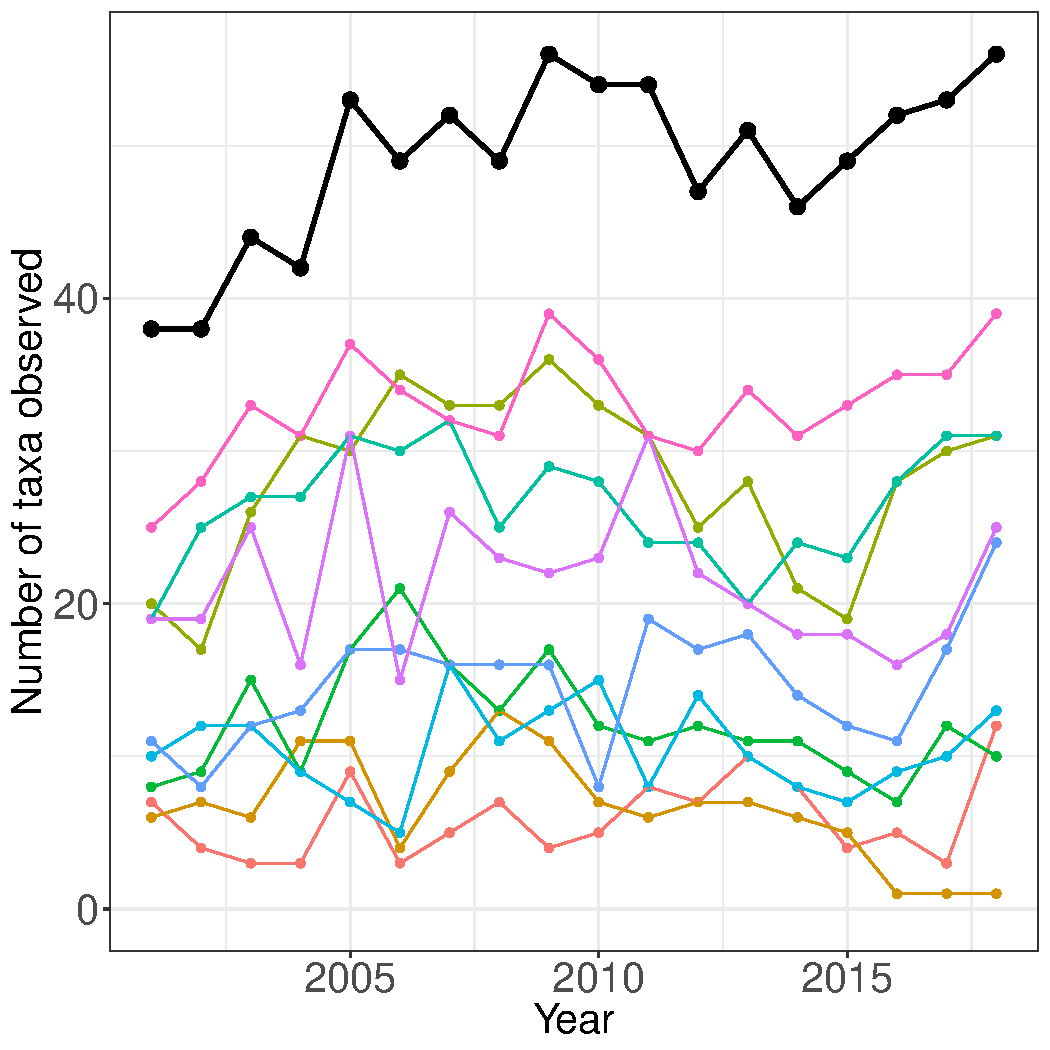
\includegraphics[scale = 0.4]{sbc-sessileInverts-castorani_num_taxa_over_time.pdf}
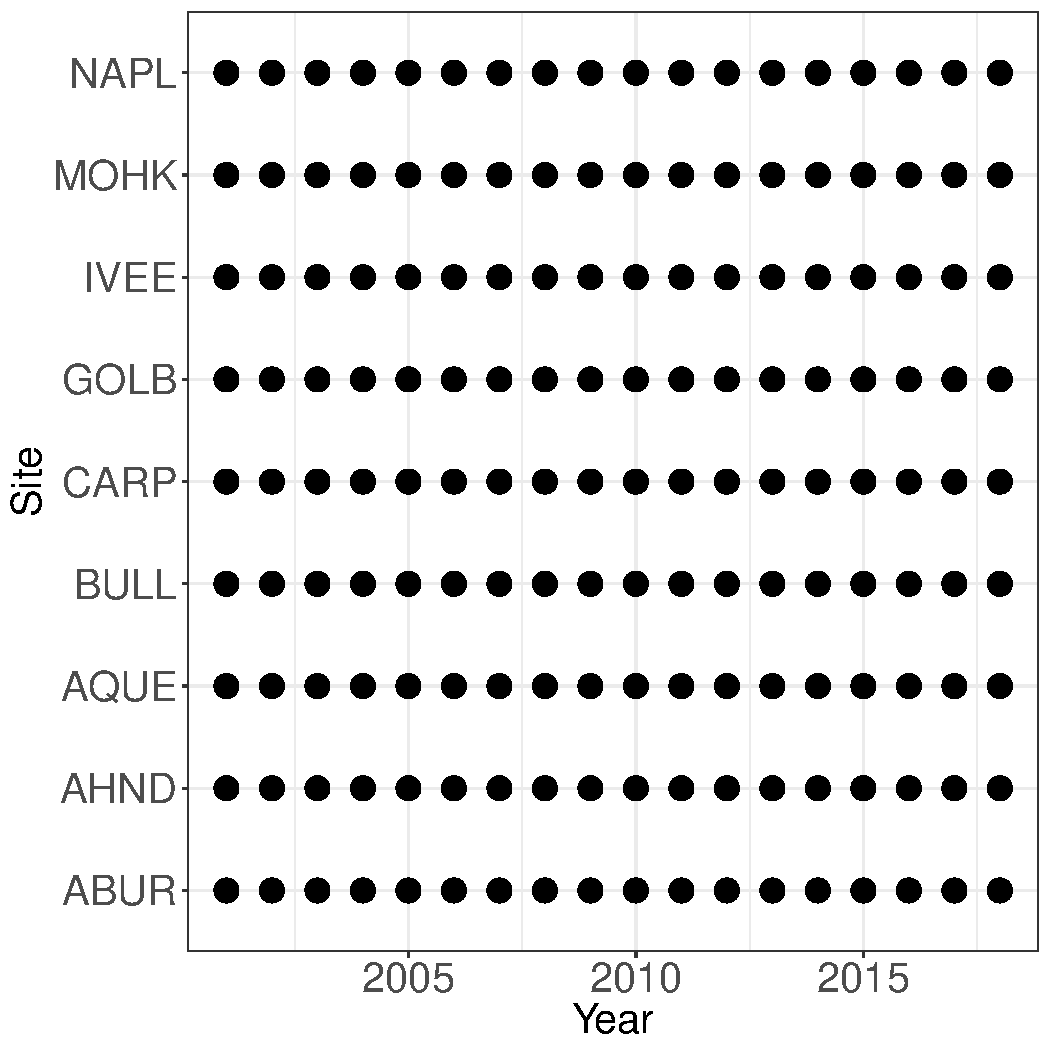
\includegraphics[scale = 0.4]{sbc-sessileInverts-castorani_spatiotemporal_sampling_effort.pdf}
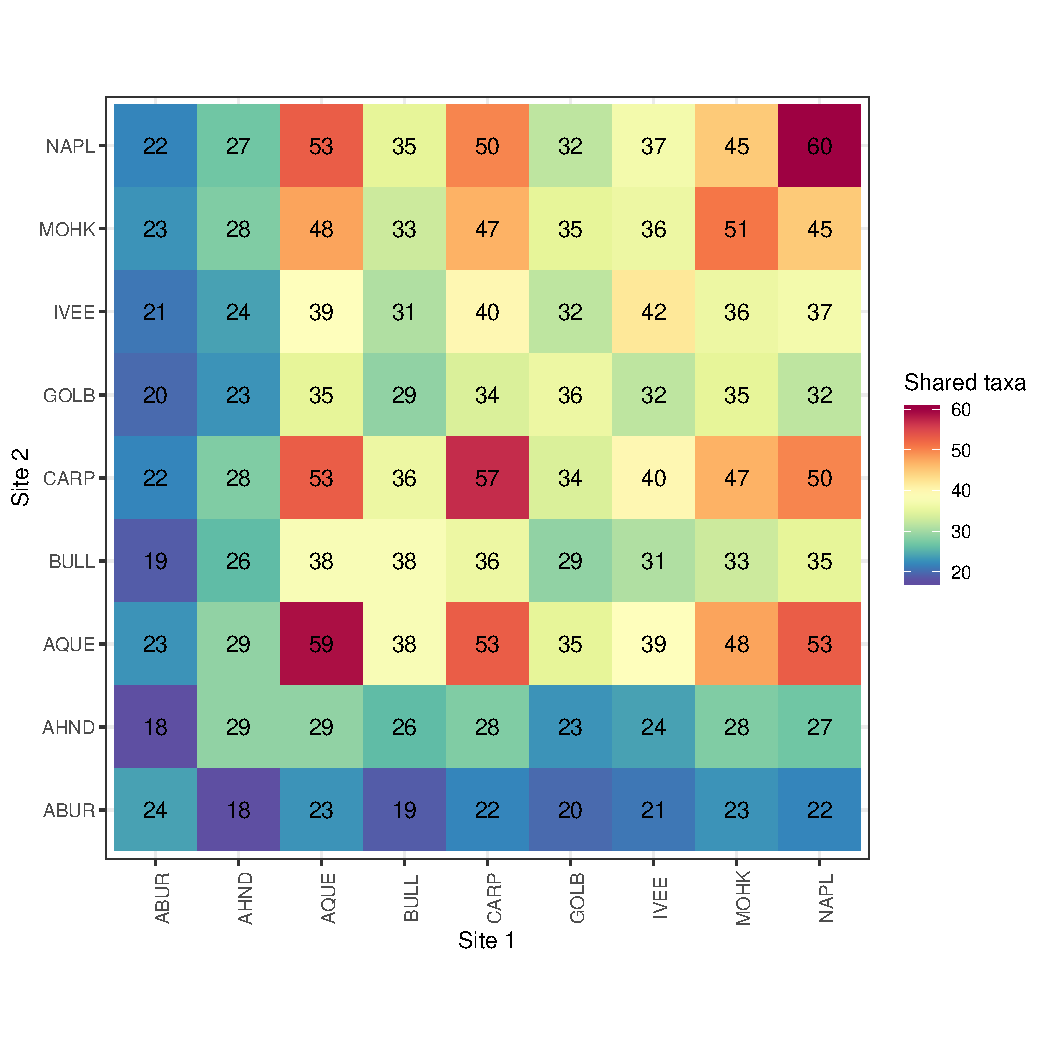
\includegraphics[scale = 0.4]{sbc-sessileInverts-castorani_spp_shared.pdf}
\caption{{\bf SBC-sessile invertebrates:} Species accumulation curves (top left),  annual richness (top right), sampling effort (bottom left), and number of shared species (bottom right)  for 70 sessile invertebrate taxa observed at 11 plots in the Santa Barbara Channel LTER (2001-2016). The black lines represent total site-level values across all plots.}
\label{sbc-sessileInverts}
\end{figure}

\subsection {sbc-survey-mobile-inverts}
{\bf Waiting for updated data to be archived on EDI.}
Two of the eleven sites were initiated in the third year of study.
I think we should remove the two sites.
Data are shown in Figure \ref{sbc-mobileInverts}

\begin{figure}[h!]
\centering
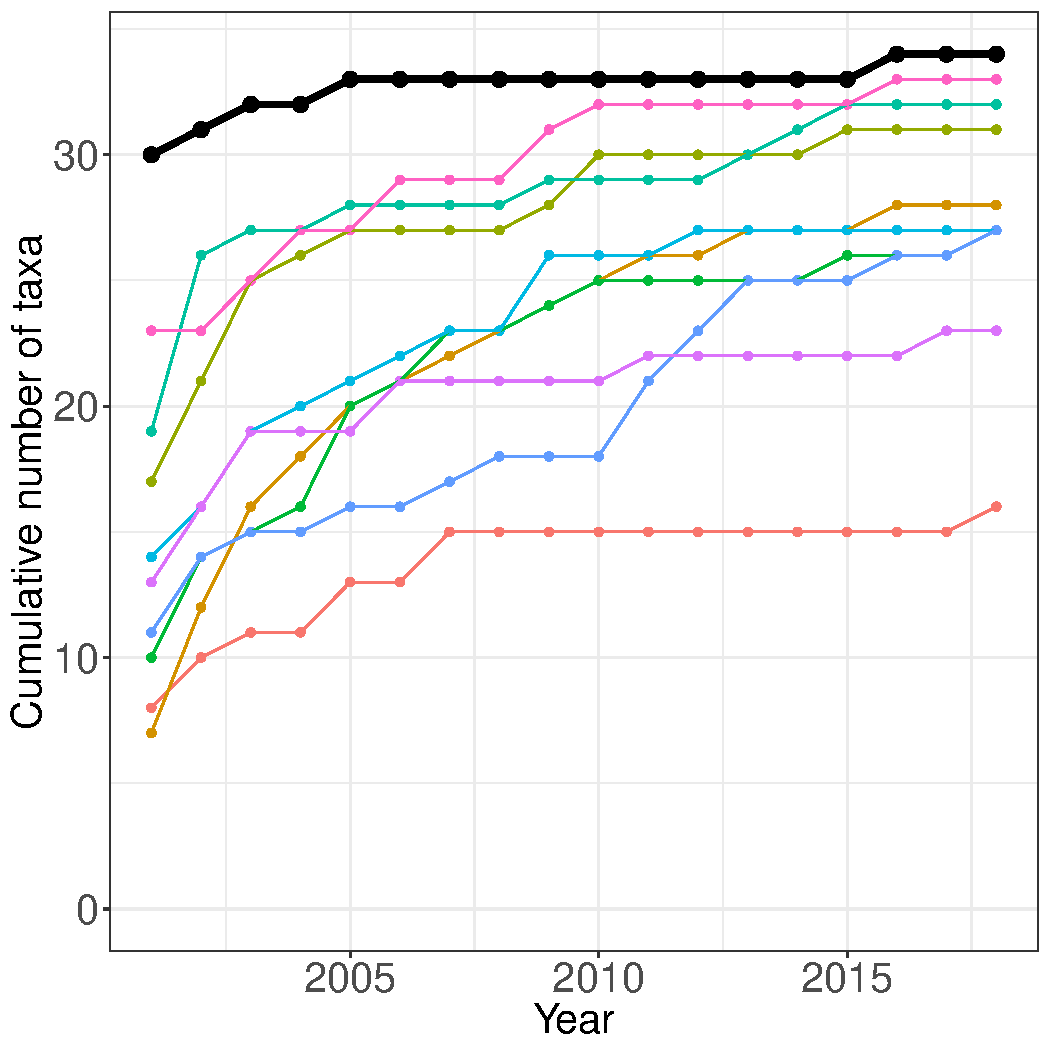
\includegraphics[scale = 0.4]{sbc-mobileInverts-castorani_species_accumulation_curve.pdf}
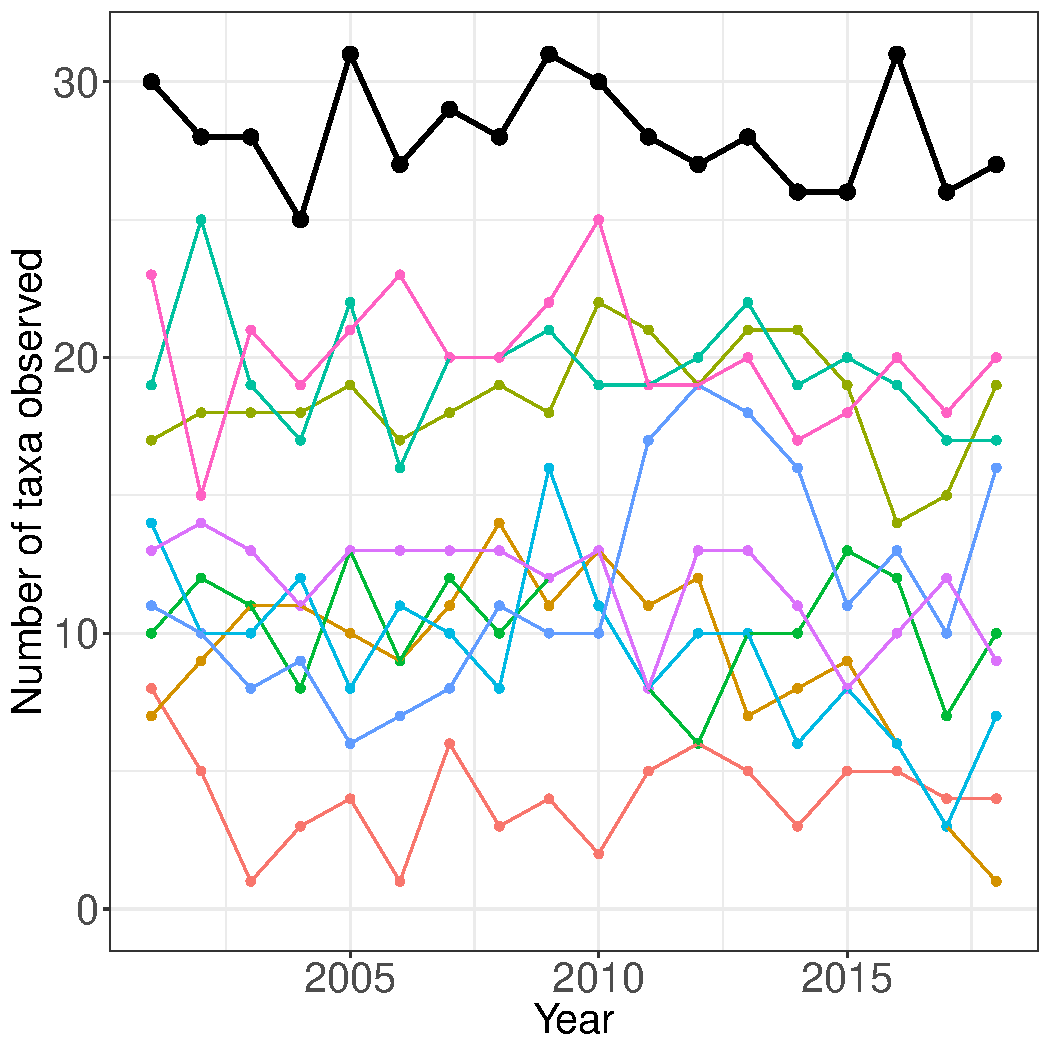
\includegraphics[scale = 0.4]{sbc-mobileInverts-castorani_num_taxa_over_time.pdf}
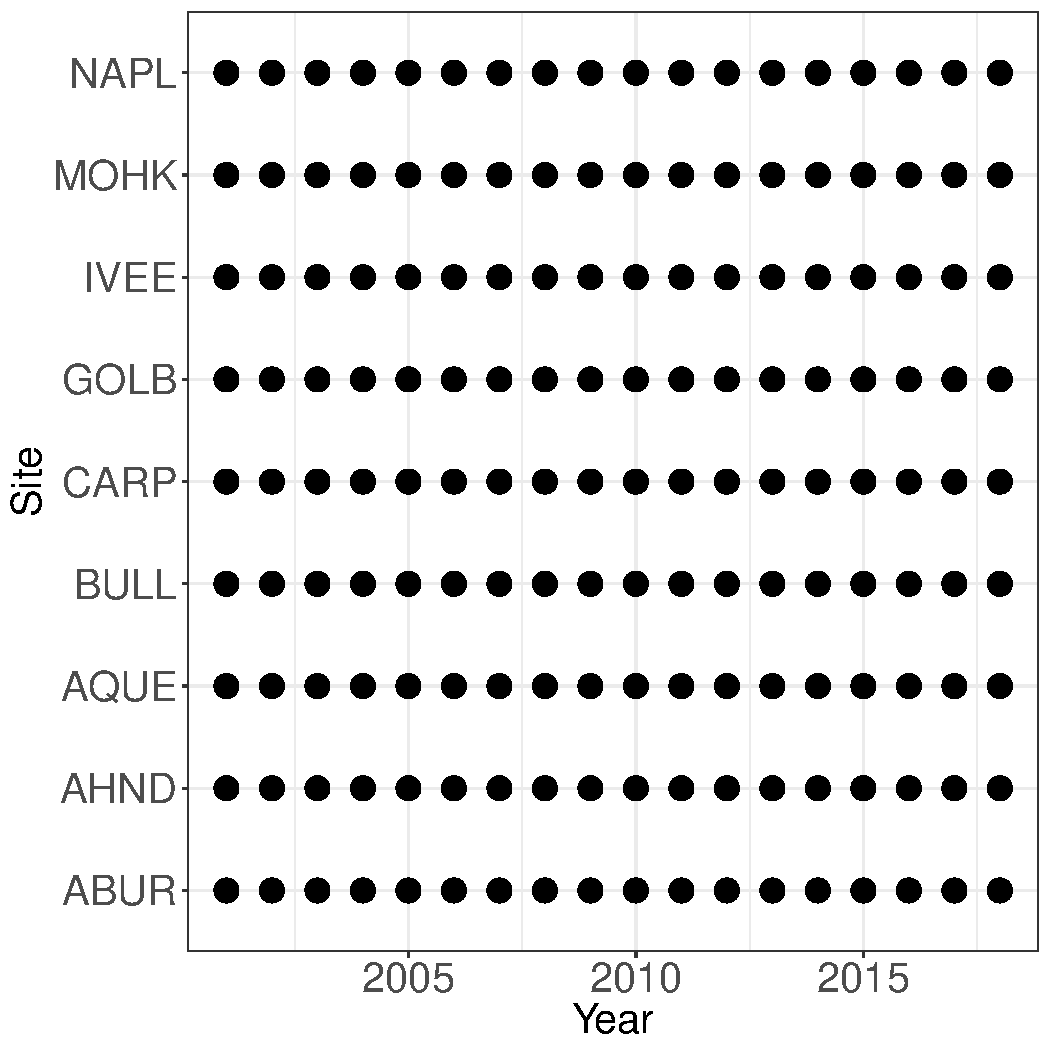
\includegraphics[scale = 0.4]{sbc-mobileInverts-castorani_spatiotemporal_sampling_effort.pdf}
\caption{{\bf SBC-mobile invertebrates:} Species accumulation curves (top left),  annual richness (top right), and sampling effort (bottom)  for 36 mobile invertebrate taxa observed at 11 plots in the Santa Barbara Channel LTER (2001-2016). The black lines represent total site-level values across all plots.}
\label{sbc-mobileInverts}
\end{figure}

\begin{figure}[h!]
\centering
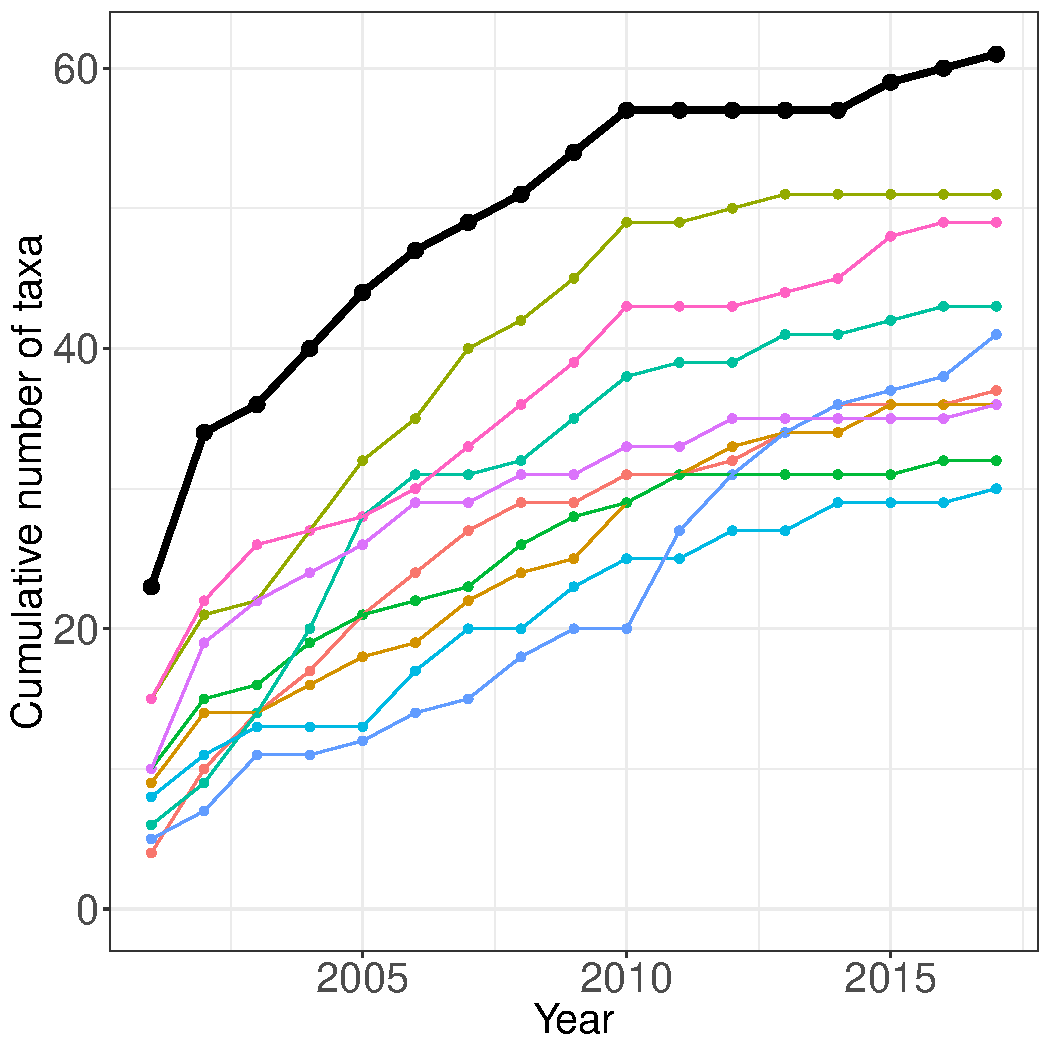
\includegraphics[scale = 0.4]{sbc-fish-castorani_species_accumulation_curve.pdf}
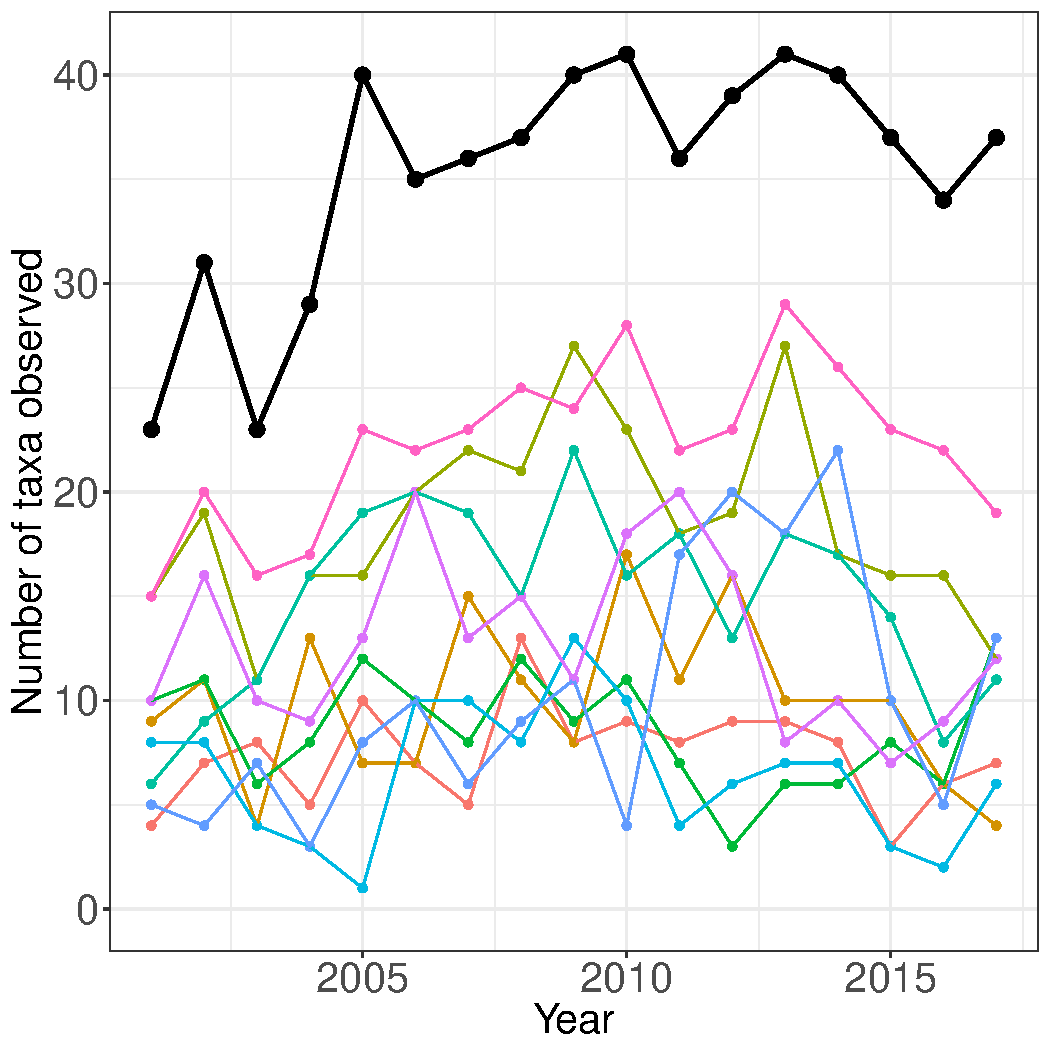
\includegraphics[scale = 0.4]{sbc-fish-castorani_num_taxa_over_time.pdf}
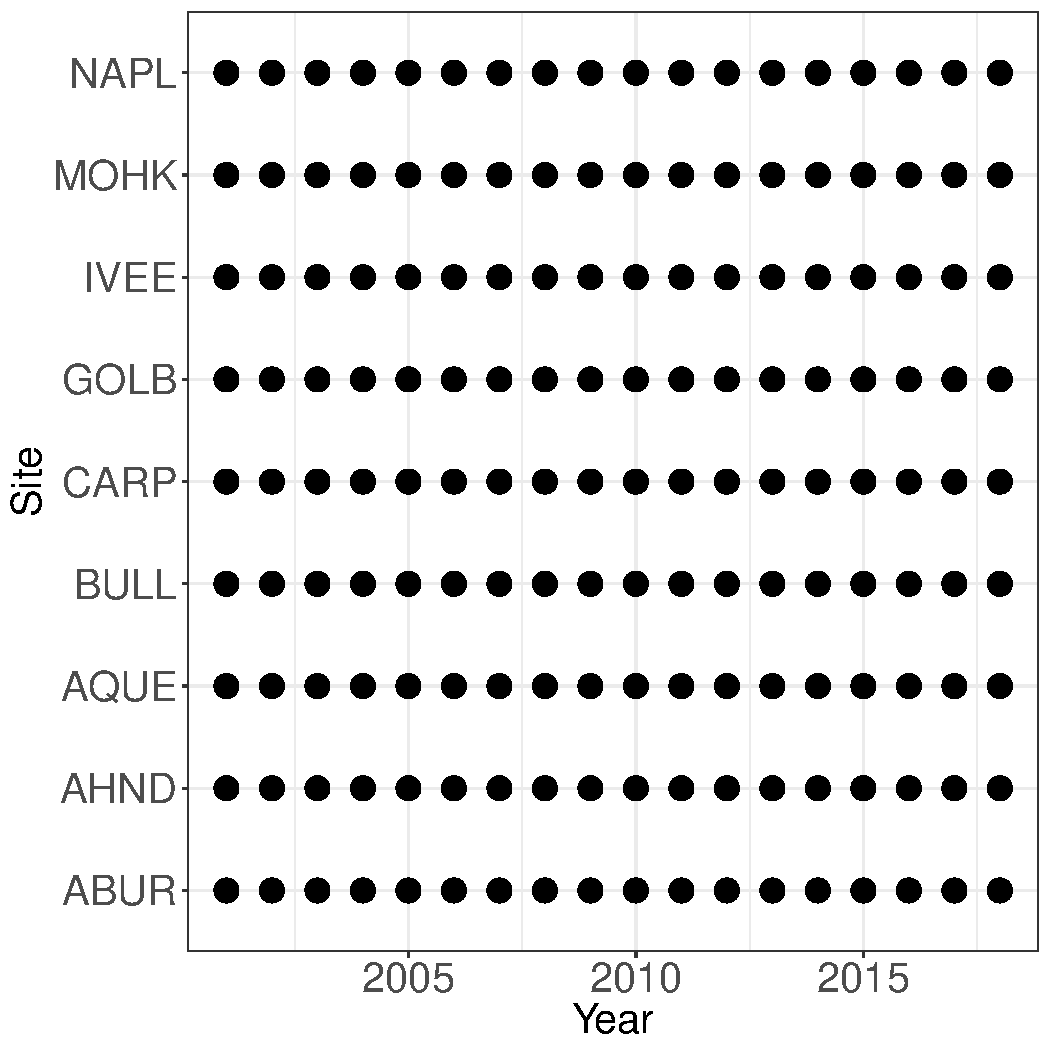
\includegraphics[scale = 0.4]{sbc-fish-castorani_spatiotemporal_sampling_effort.pdf}
%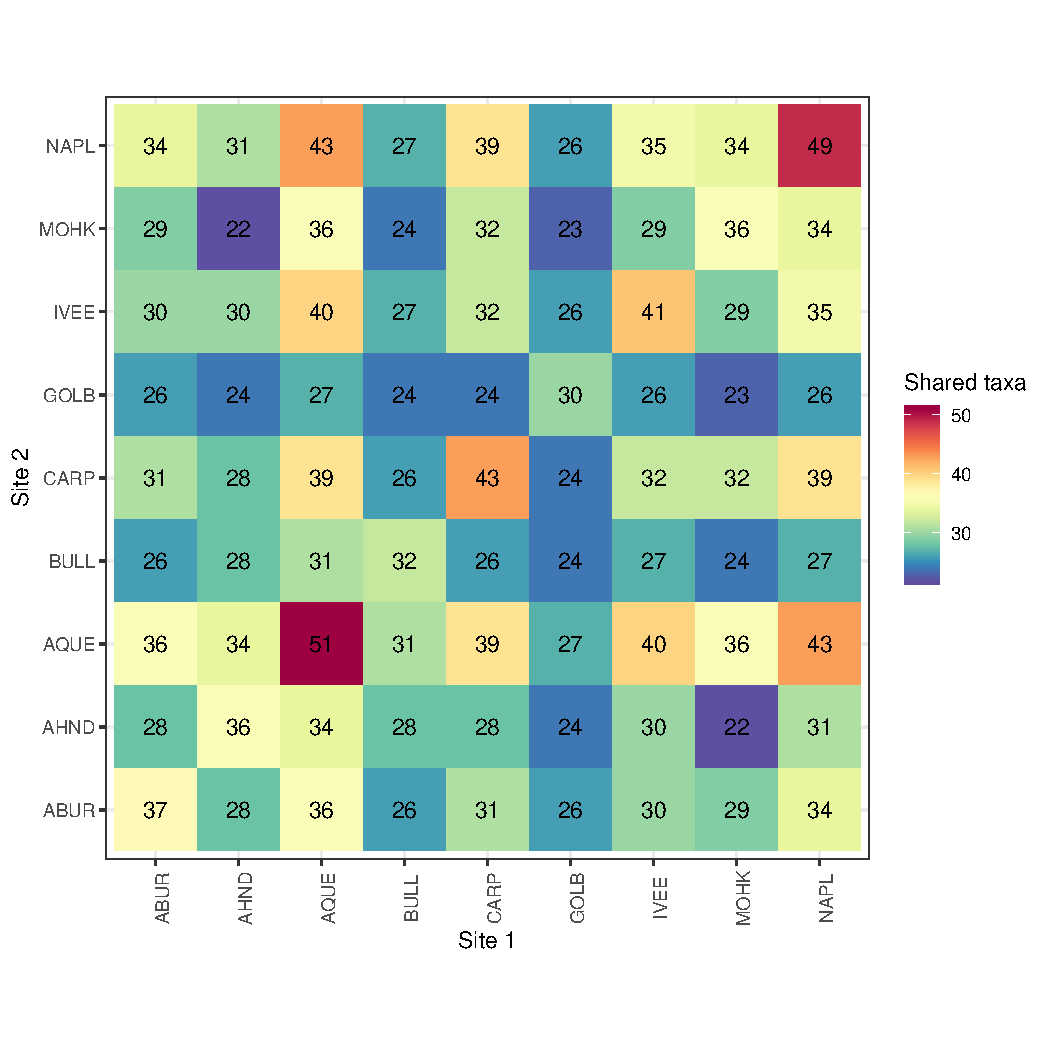
\includegraphics[scale = 0.4]{sbc-fish-castorani_spp_shared.pdf}
\caption{{\bf SBC-fish:} Species accumulation curves (top left),  annual richness (top right), and sampling effort (bottom)  for 64 fish species observed at 11 plots in the Santa Barbara Channel LTER (2001-2016). The black lines represent total site-level values across all plots.}
\label{sbc-fish}
\end{figure}

\subsection {mcr-inverts}
{\bf Need to get updated data. Need to separate by habitat. Needs data package citation.}
Data were downloaded from EDI (knb-lter-mcr.7.28).
Data were aggregated across habitats and transects.
Thus each of the six sites contains data from very different habitats lumped together (back, fringing, outer reefs) and there is likely very little overlap in the species found in each habitat. 
This is different than the other datasets, and it would be good to discuss whether or not to separate by habitat.
Non-relevant taxa and taxa observed outside the quadrat were removed from the dataset.
Abundance was averaged across subplots, transects, and habitats for each species at each site in each year.
Data are in Figure \ref{mcr-inverts}.
It's unclear whether these are mobile inverts, sessile inverts, or both (need to know for comparison with SBC).
\begin{figure}[h!]
\centering
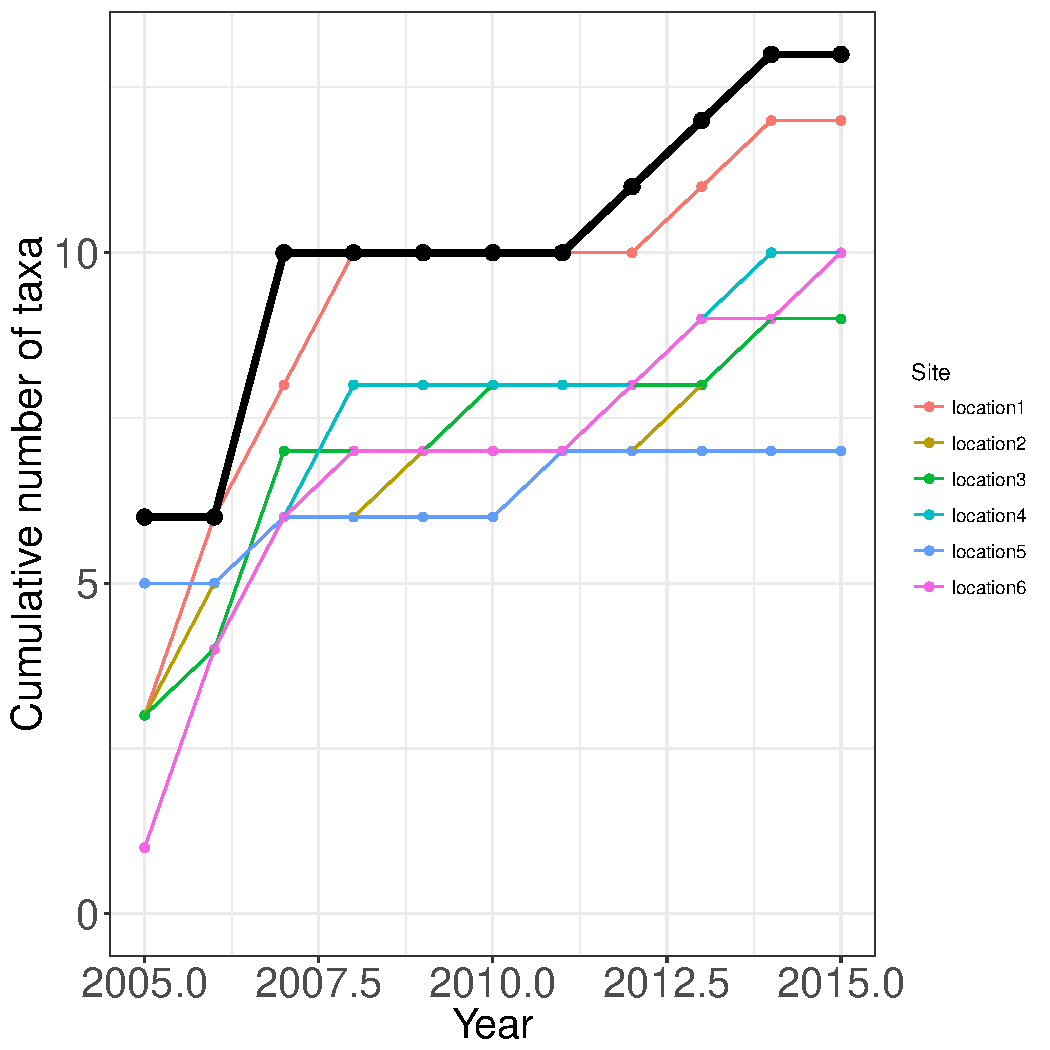
\includegraphics[scale = 0.4]{mcr-inverts-castorani_species_accumulation_curve.pdf}
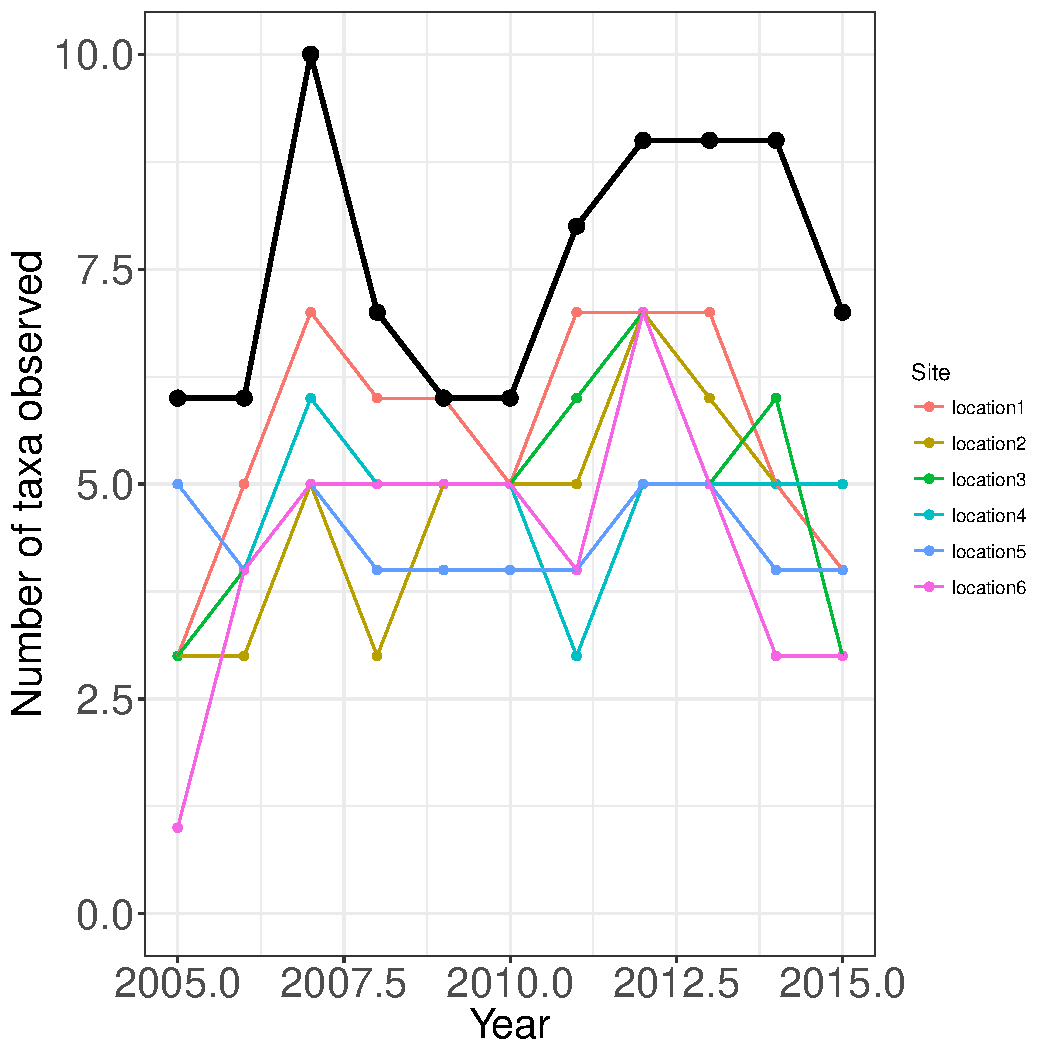
\includegraphics[scale = 0.4]{mcr-inverts-castorani_num_taxa_over_time.pdf}
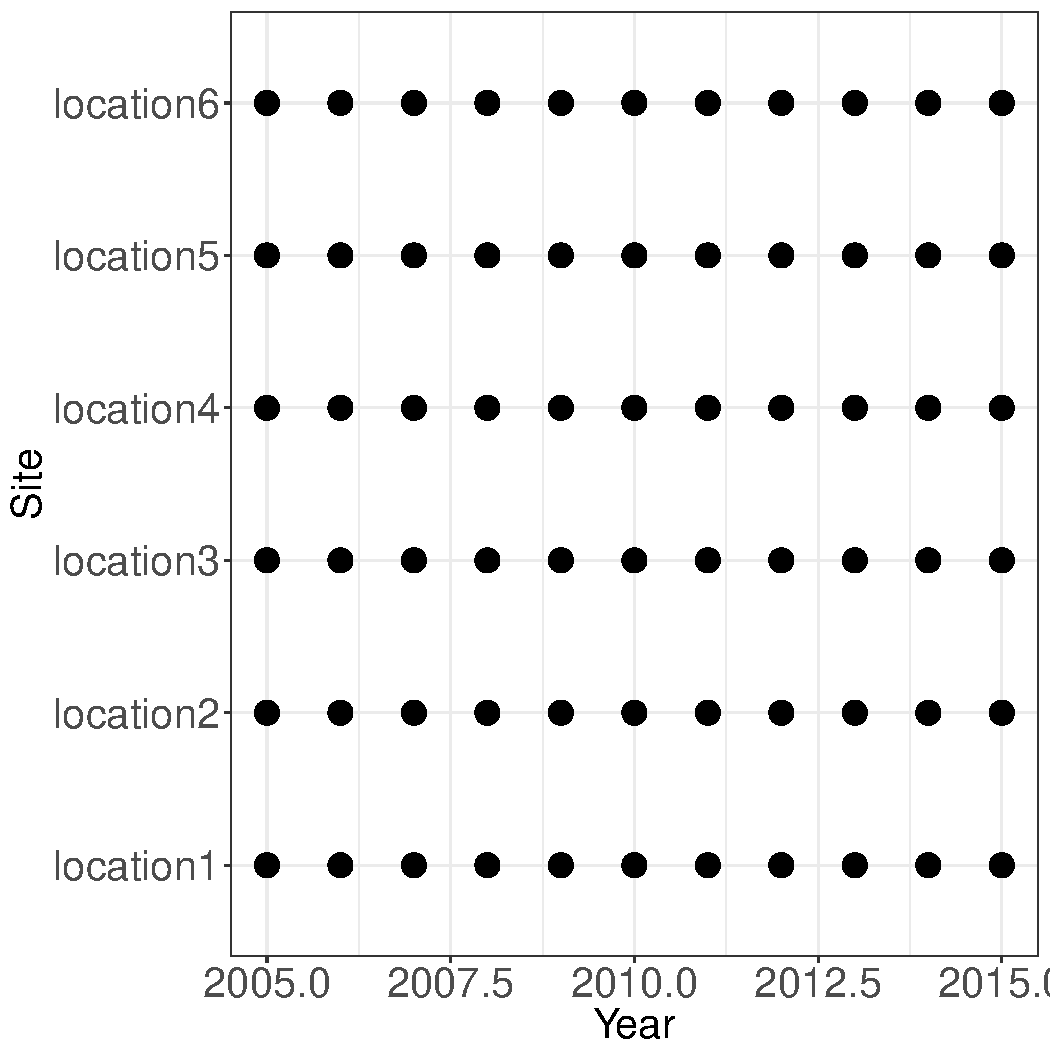
\includegraphics[scale = 0.4]{mcr-inverts-castorani_spatiotemporal_sampling_effort.pdf}
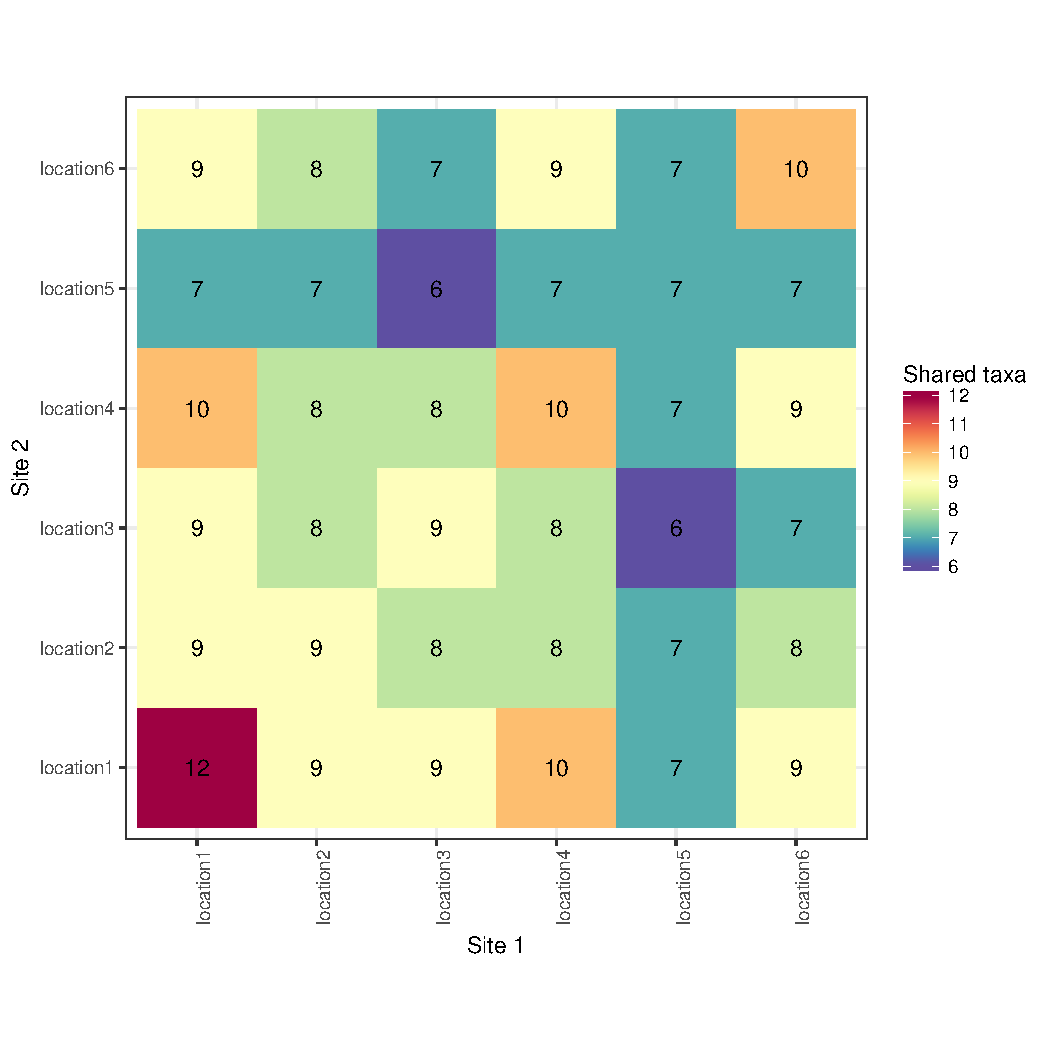
\includegraphics[scale = 0.4]{mcr-inverts-castorani_spp_shared.pdf}
\caption{{\bf MCR-inverts:} Species accumulation curves (top left),  annual richness (top right), and sampling effort (bottom)  for 13 invertebrate taxa observed at six sites on Moorea coral reef LTER (2006-2015). The black lines represent total site-level values across all plots.}
\label{mcr-inverts}
\end{figure}


\subsection {mcr-fish}
{\bf Updated data in ecocomdp format on EDI. Need to prepare it for this analysis. Need to separate by habitat. Needs data package citation.}
%Data were downloaded from EDI (knb-lter-mcr.6.54).
Data were aggregated across habitats and transects.
Thus each of the six sites contains data from very different habitats lumped together (backreef, forereef, fringing) and there is likely very little overlap in the species found in each habitat. 
This is different than the other datasets, and it would be good to discuss whether or not to separate by habitat.
Non-relevant taxa codes (e.g. ``No fish present") were removed from the dataset.
Abundance was recorded as dry biomass per 250 $m^2$, averaged across subplots, transects, and habitats for each species at each site in each year.
Data are in Figure \ref{mcr-fish}.
Six extra locations in forereef habitats were sampled in 2015.
These appear to be in addition to the four transects per habitat per site performed as part of the long term data collections, and thus they were removed from the dataset prior to analysis.
\begin{figure}[h!]
\centering
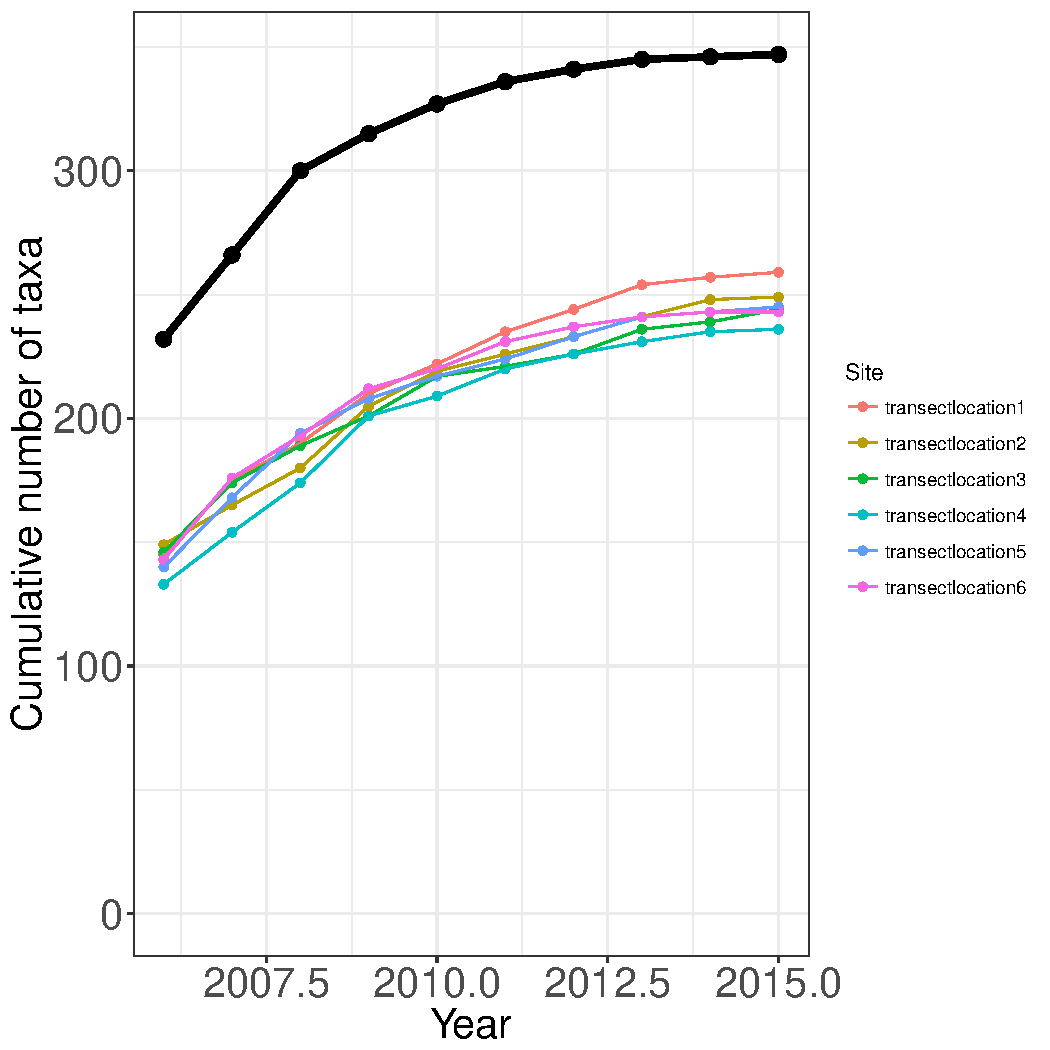
\includegraphics[scale = 0.4]{mcr-fish-castorani_species_accumulation_curve.pdf}
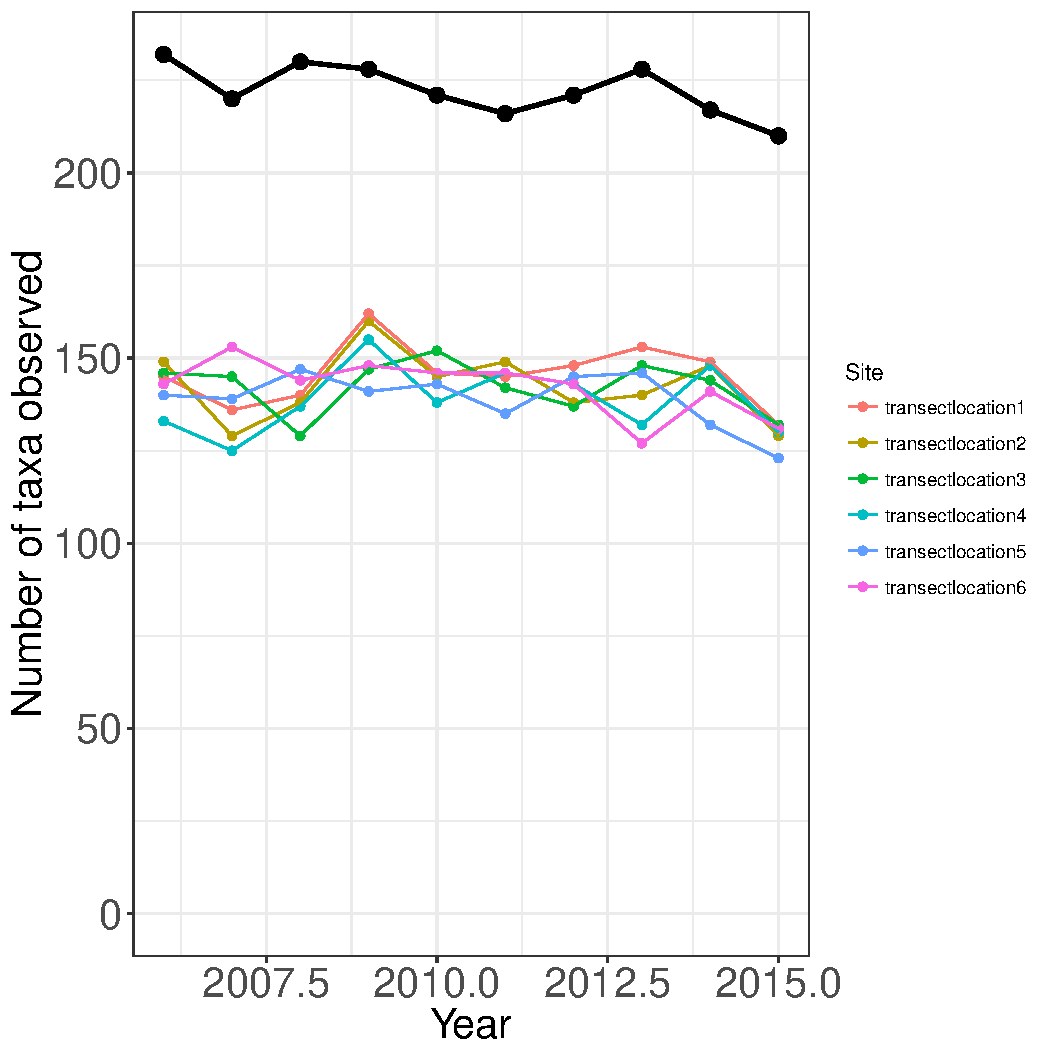
\includegraphics[scale = 0.4]{mcr-fish-castorani_num_taxa_over_time.pdf}
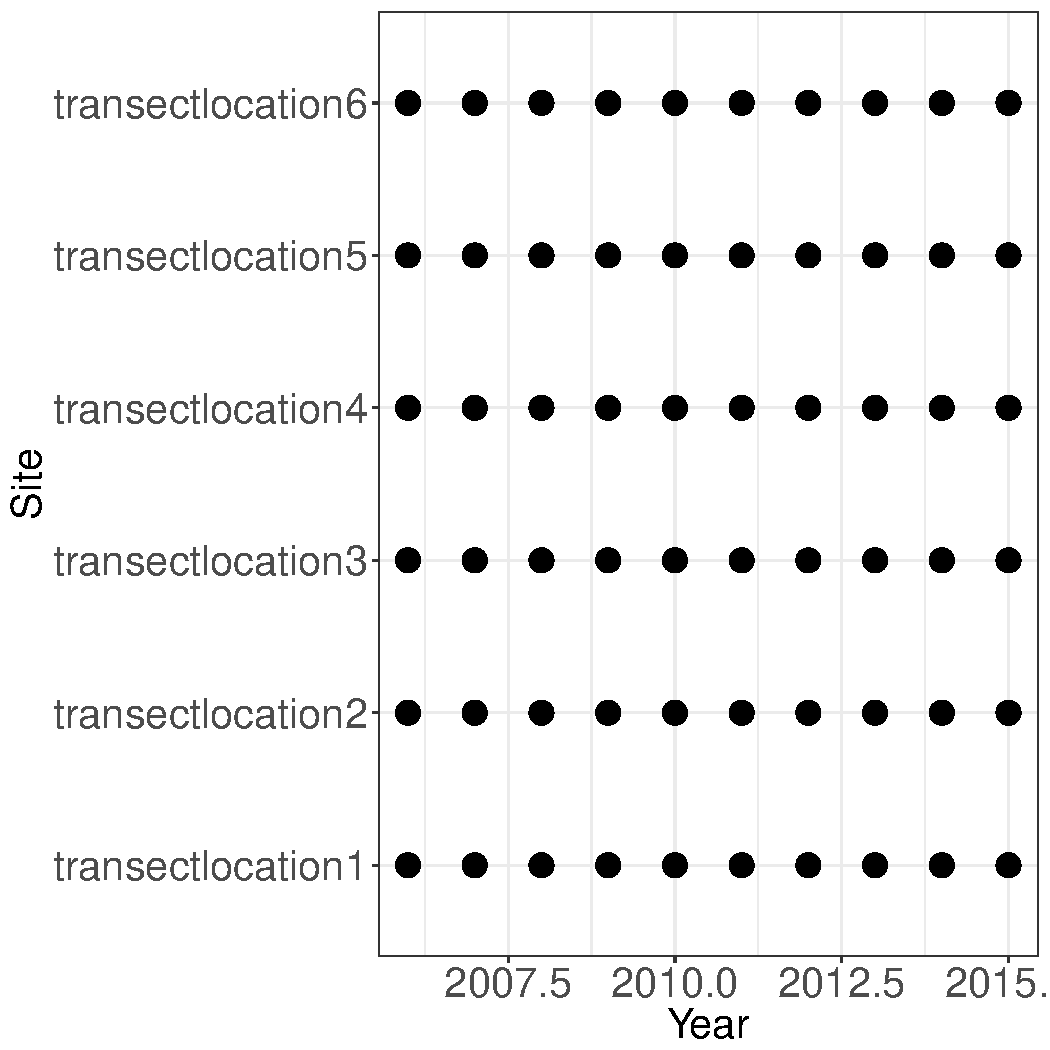
\includegraphics[scale = 0.4]{mcr-fish-castorani_spatiotemporal_sampling_effort.pdf}
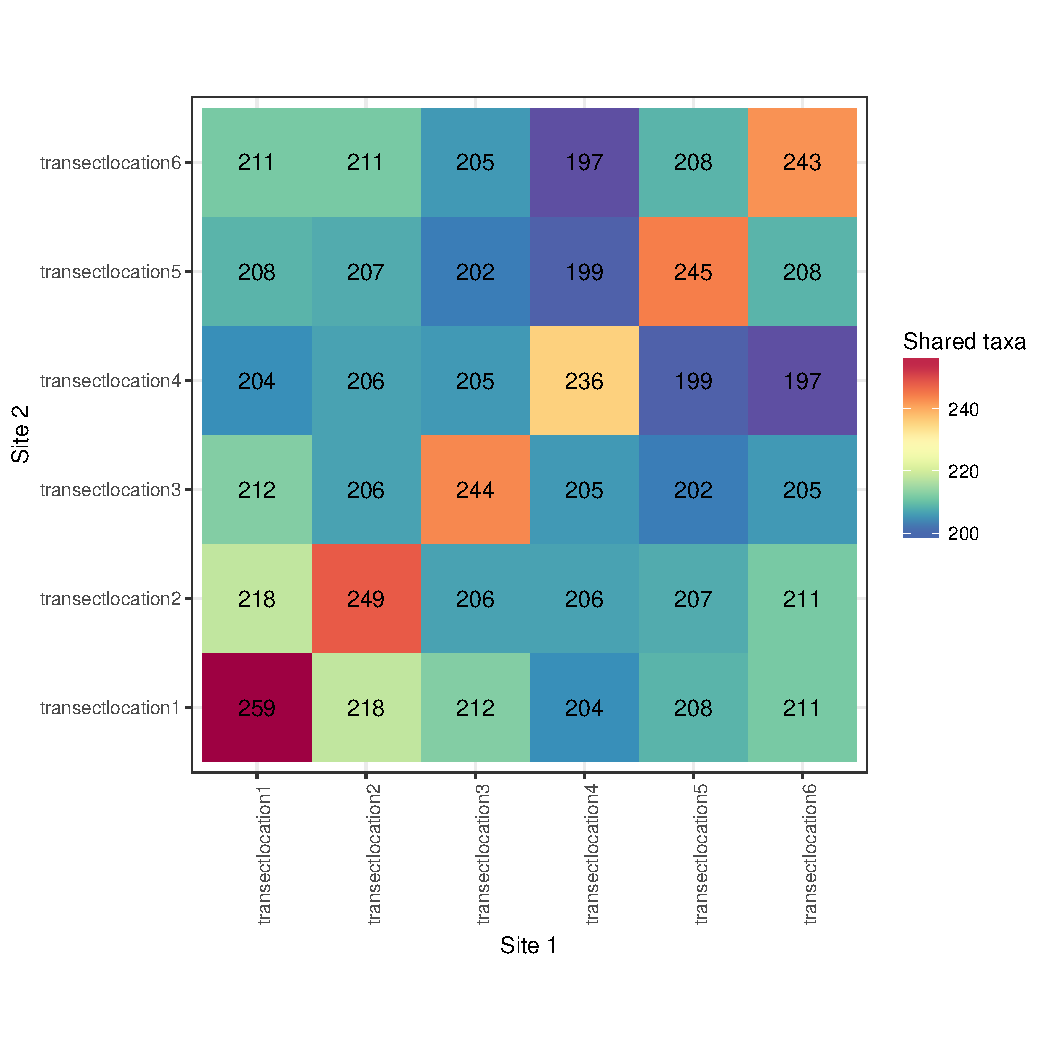
\includegraphics[scale = 0.4]{mcr-fish-castorani_spp_shared.pdf}
\caption{{\bf MCR-fish:} Species accumulation curves (top left),  annual richness (top right), and sampling effort (bottom)  for 377 fish taxa observed at six sites on Moorea coral reef LTER (2006-2015). The black lines represent total site-level values across all plots.}
\label{mcr-fish}
\end{figure}


\subsection {mcr-coral}
{\bf Need to get updated data. Need to separate by habitat. Needs data package citation.}
Data were downloaded from EDI \citep{mcr-coral}.
The corals are identified to the genus level.
Data were aggregated across habitats and transects.
Thus each of the six sites contains data from very different habitats lumped together (back, fringing, outer reefs) and there is likely very little overlap in the species found in each habitat. 
This is different than the other datasets, and it would be good to discuss whether or not to separate by habitat.
Non-relevant taxa were removed from the dataset.
Abundance was averaged across subplots, transects, and habitats for each species at each site in each year.
Data are in Figure \ref{mcr-coral}.
\begin{figure}[h!]
\centering
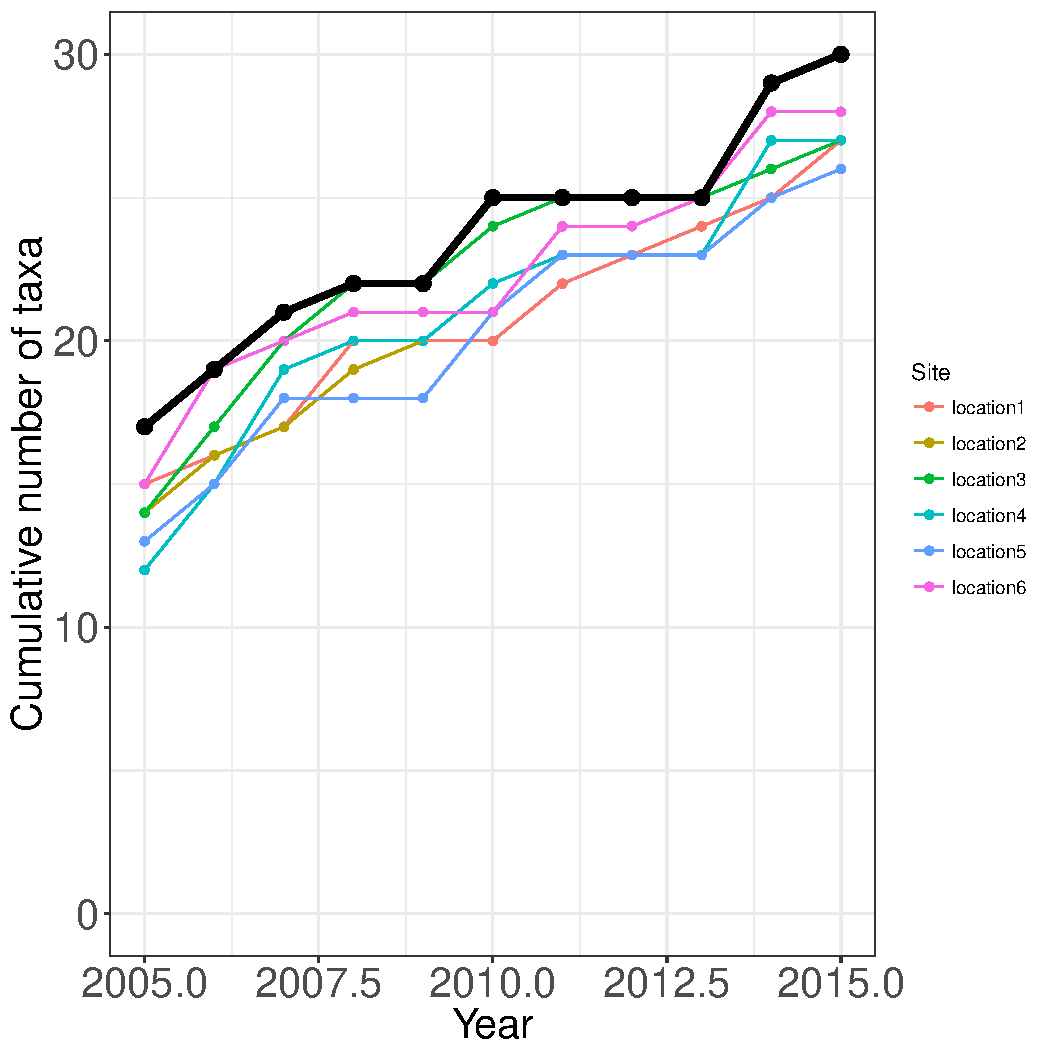
\includegraphics[scale = 0.4]{mcr-coral-castorani_species_accumulation_curve.pdf}
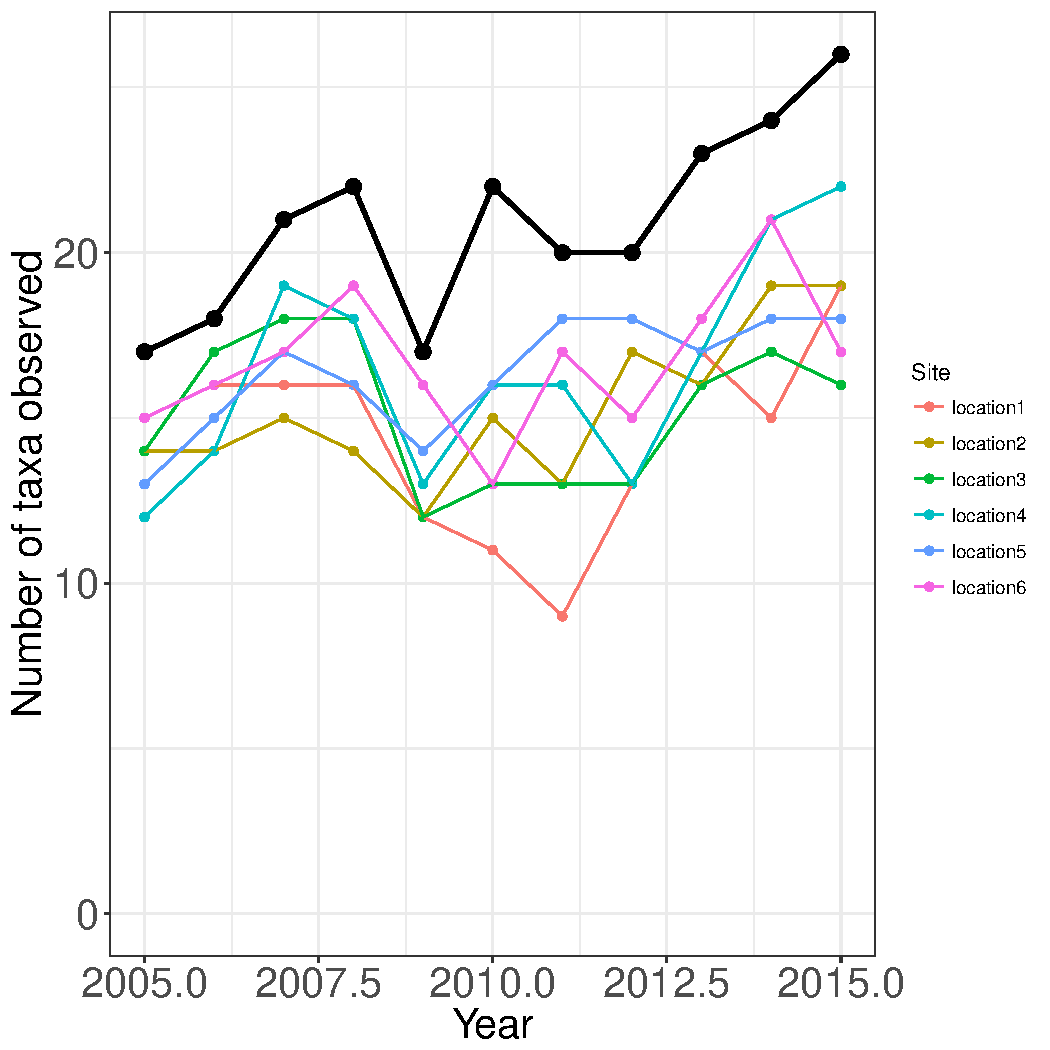
\includegraphics[scale = 0.4]{mcr-coral-castorani_num_taxa_over_time.pdf}
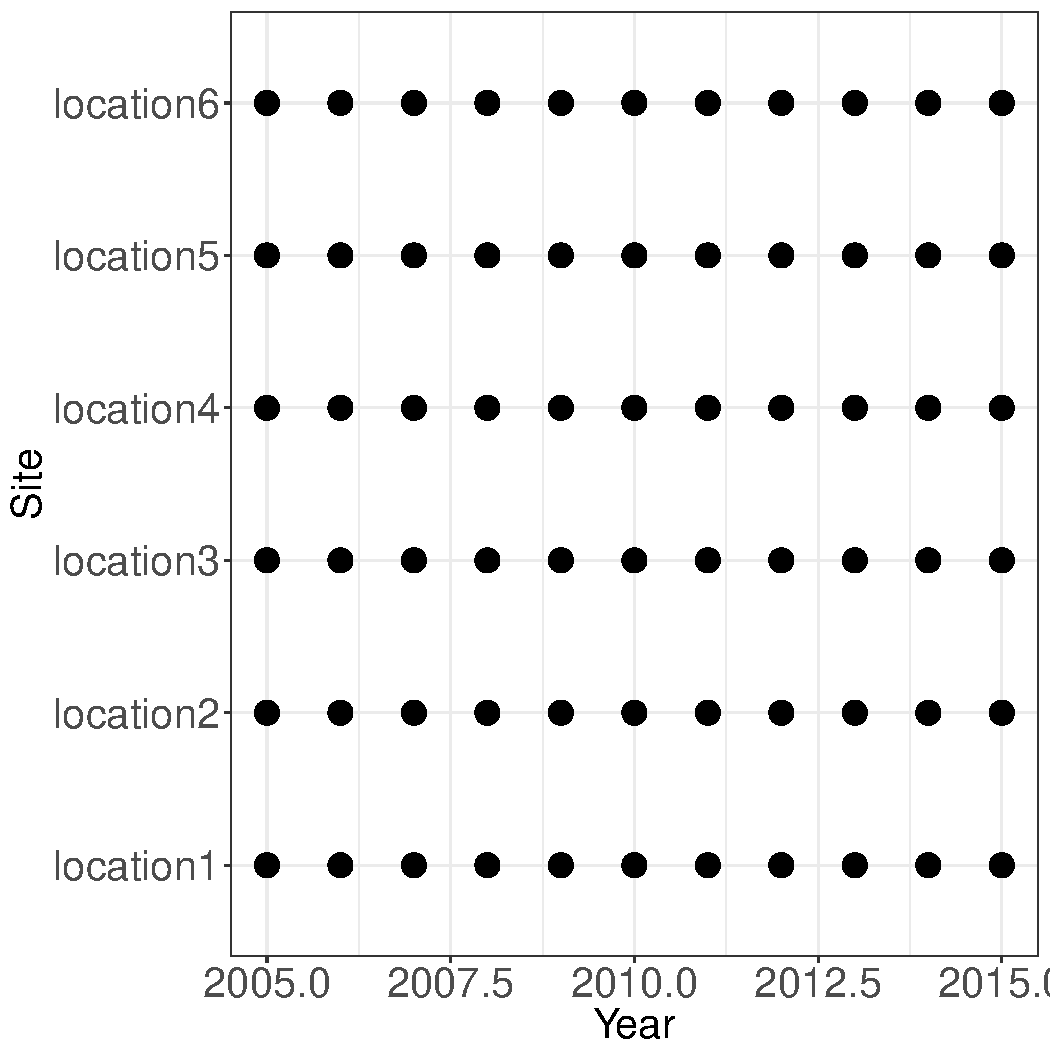
\includegraphics[scale = 0.4]{mcr-coral-castorani_spatiotemporal_sampling_effort.pdf}
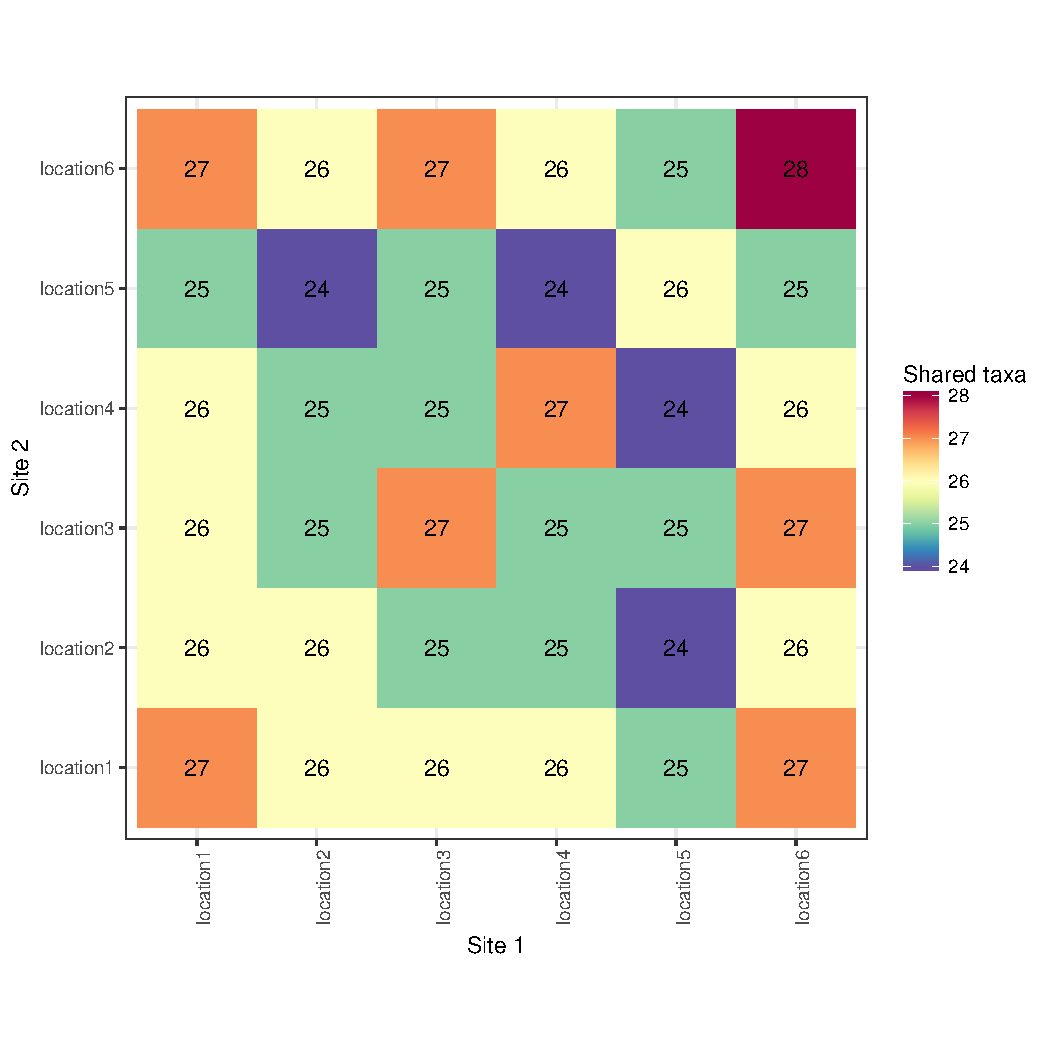
\includegraphics[scale = 0.4]{mcr-coral-castorani_spp_shared.pdf}
\caption{{\bf MCR-coral:} Species accumulation curves (top left),  annual richness (top right), and sampling effort (bottom)  for 31 coral taxa observed at six sites on Moorea coral reef LTER (2006-2015). The black lines represent total site-level values across all plots.}
\label{mcr-coral}
\end{figure}




\subsection {mcr-algae}
{\bf Need to get updated data. Need to separate by habitat. Needs data package citation.}
Data were downloaded from EDI \citep{mcr-algae}.
Data were aggregated across habitats and transects.
Thus each of the six sites contains data from very different habitats lumped together (back, fringing, outer reefs) and there is likely very little overlap in the species found in each habitat. 
This is different than the other datasets, and it would be good to discuss whether or not to separate by habitat.
Non-relevant taxa were removed from the dataset.
Abundance was averaged across subplots, transects, and habitats for each species at each site in each year.
Data are in Figure \ref{mcr-algae}.
The cumulative number of taxa was still increasing at the end of the time series.
\begin{figure}[h!]
\centering
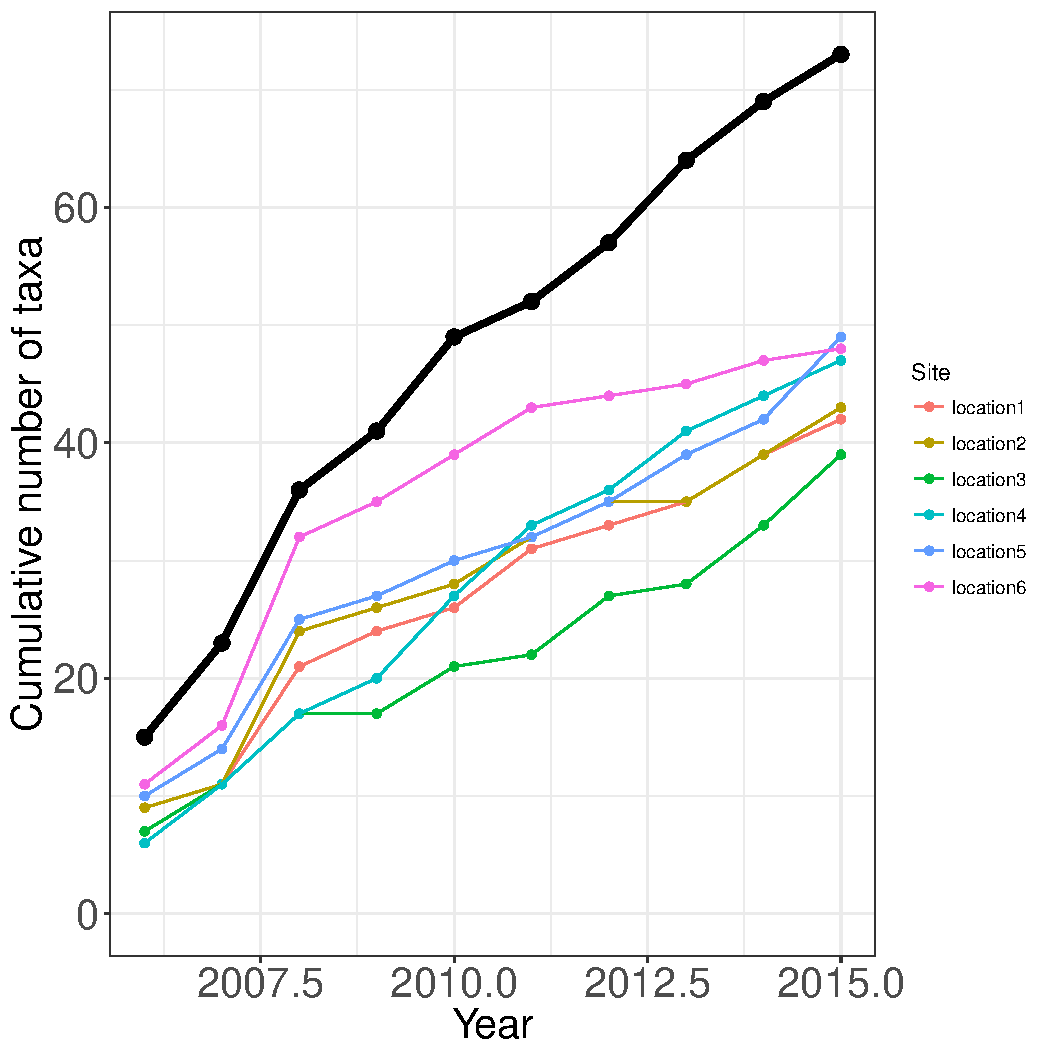
\includegraphics[scale = 0.4]{mcr-algae-castorani_species_accumulation_curve.pdf}
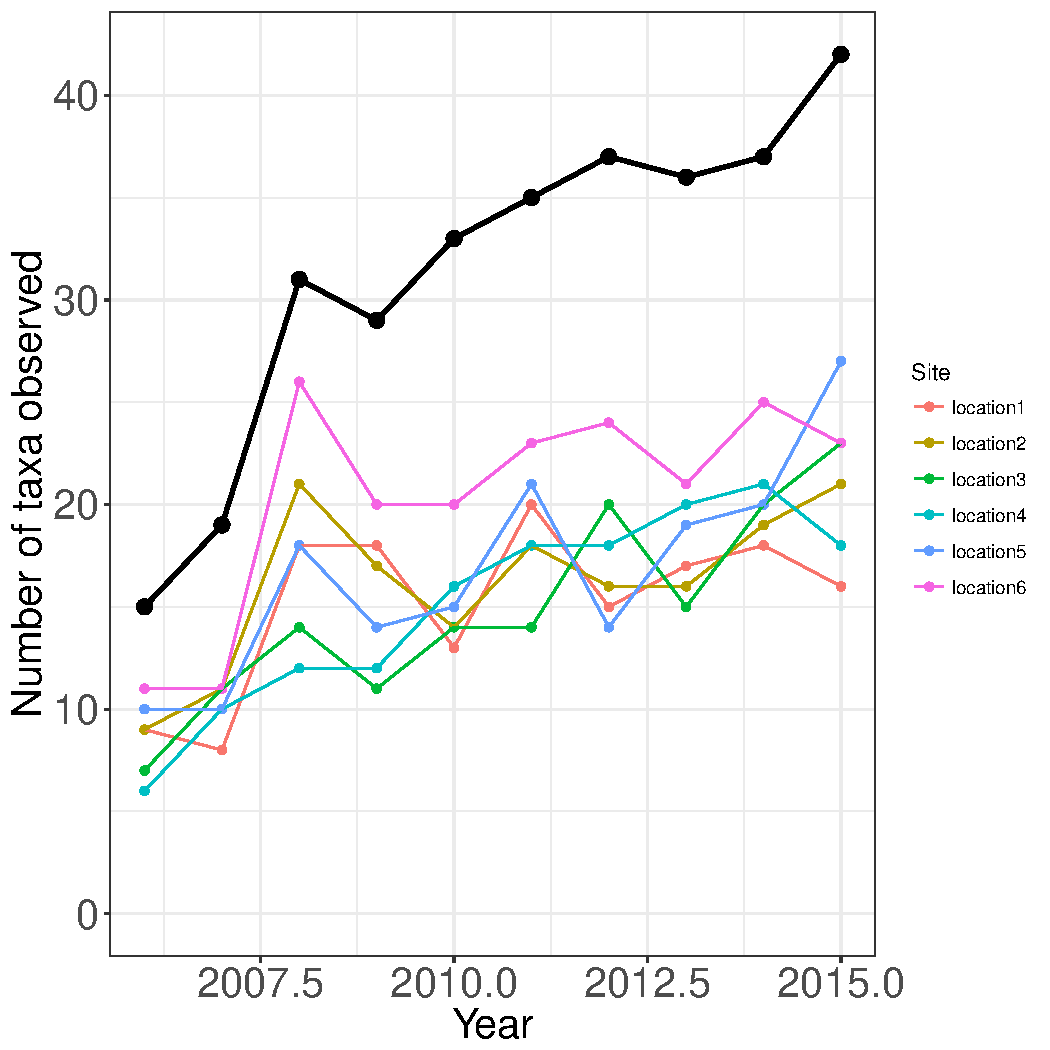
\includegraphics[scale = 0.4]{mcr-algae-castorani_num_taxa_over_time.pdf}
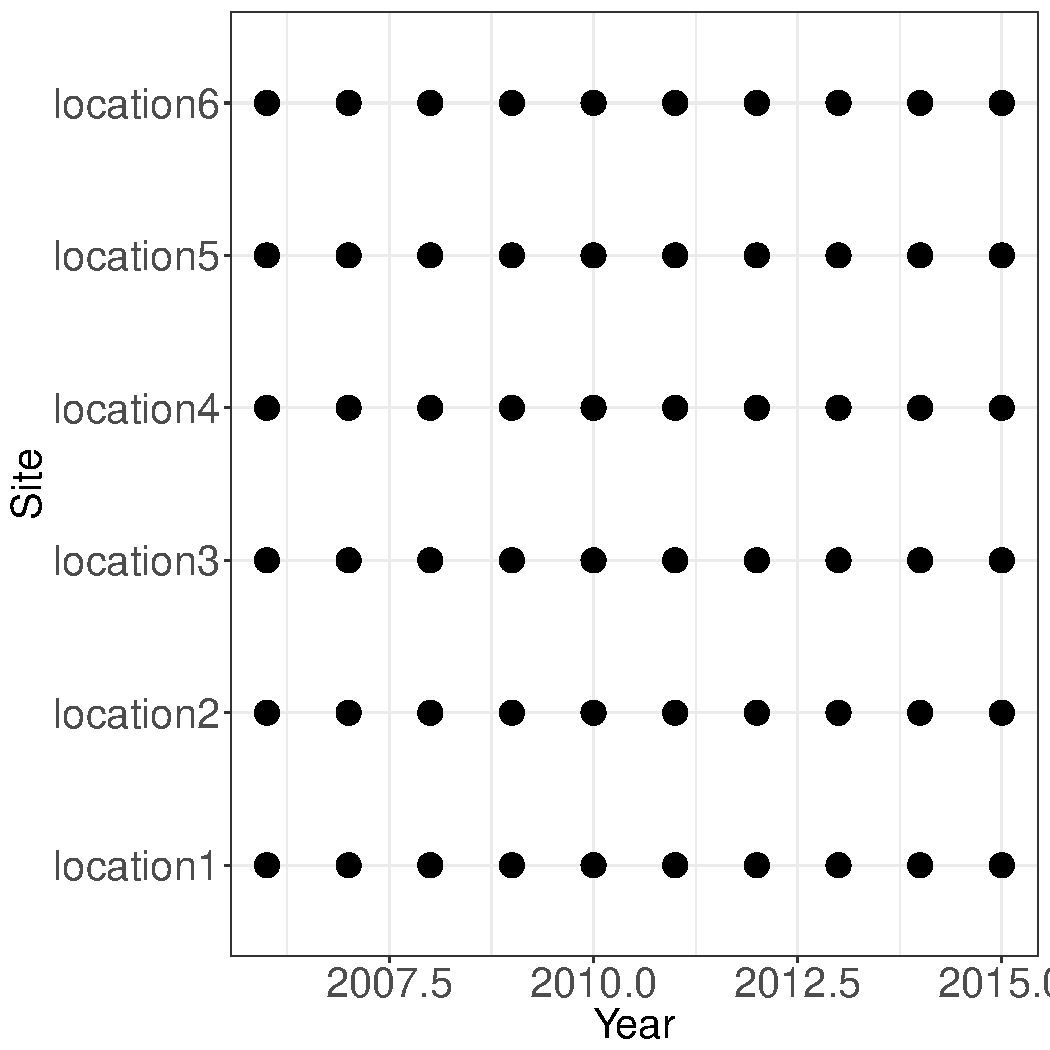
\includegraphics[scale = 0.4]{mcr-algae-castorani_spatiotemporal_sampling_effort.pdf}
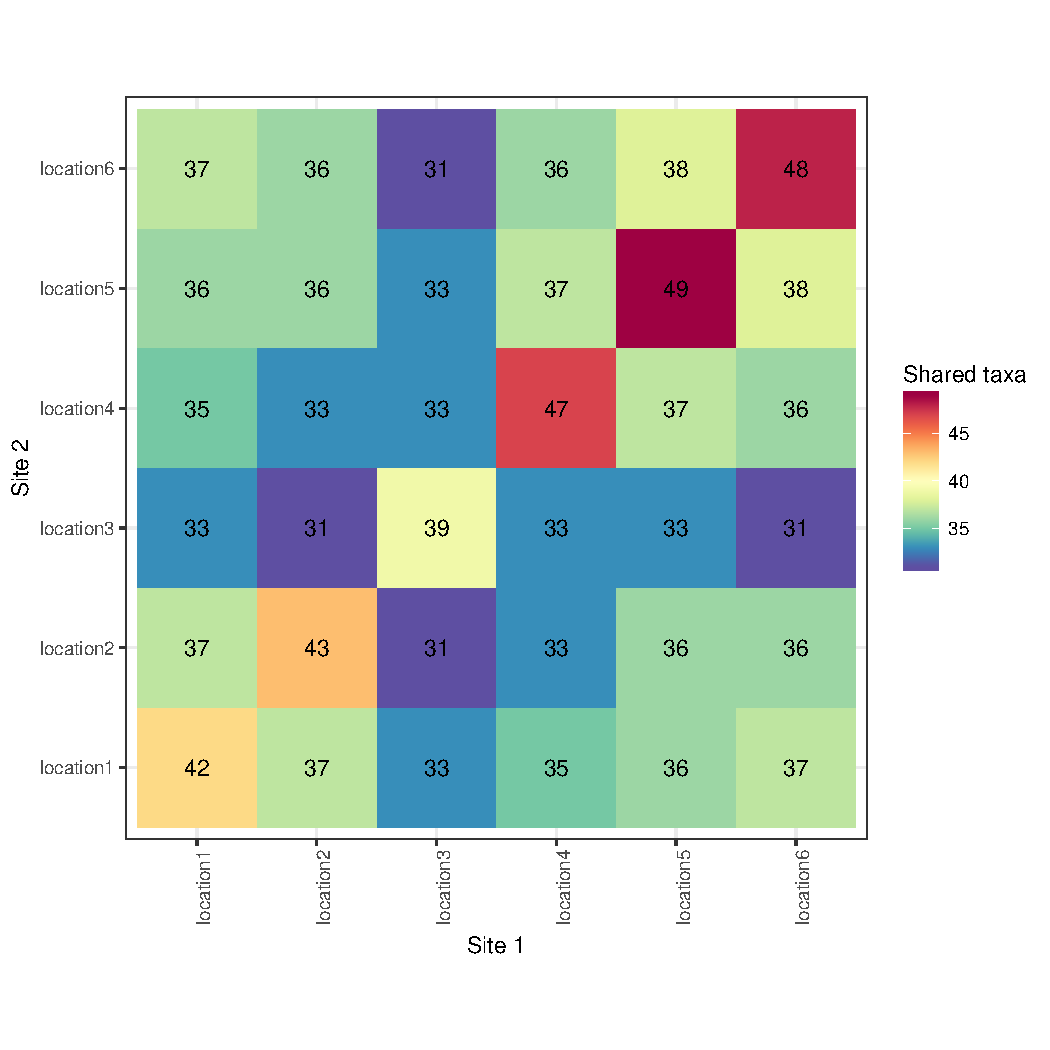
\includegraphics[scale = 0.4]{mcr-algae-castorani_spp_shared.pdf}
\caption{{\bf MCR-algae:} Species accumulation curves (top left),  annual richness (top right), and sampling effort (bottom)  for 73 algae taxa observed at six sites on Moorea coral reef LTER (2006-2015). The black lines represent total site-level values across all plots.}
\label{mcr-algae}
\end{figure}


%%%%%%%%%%%%%%%%%%%%%%
\section {Freshwater datasets}

\subsection {fce-diatoms}
Data were obtained from the PI.
Metadata and citation can be found on EDI \citep{fce-diatoms}.
Data are shown in Figure \ref{fce-diatoms}
\begin{figure}[h!]
\centering
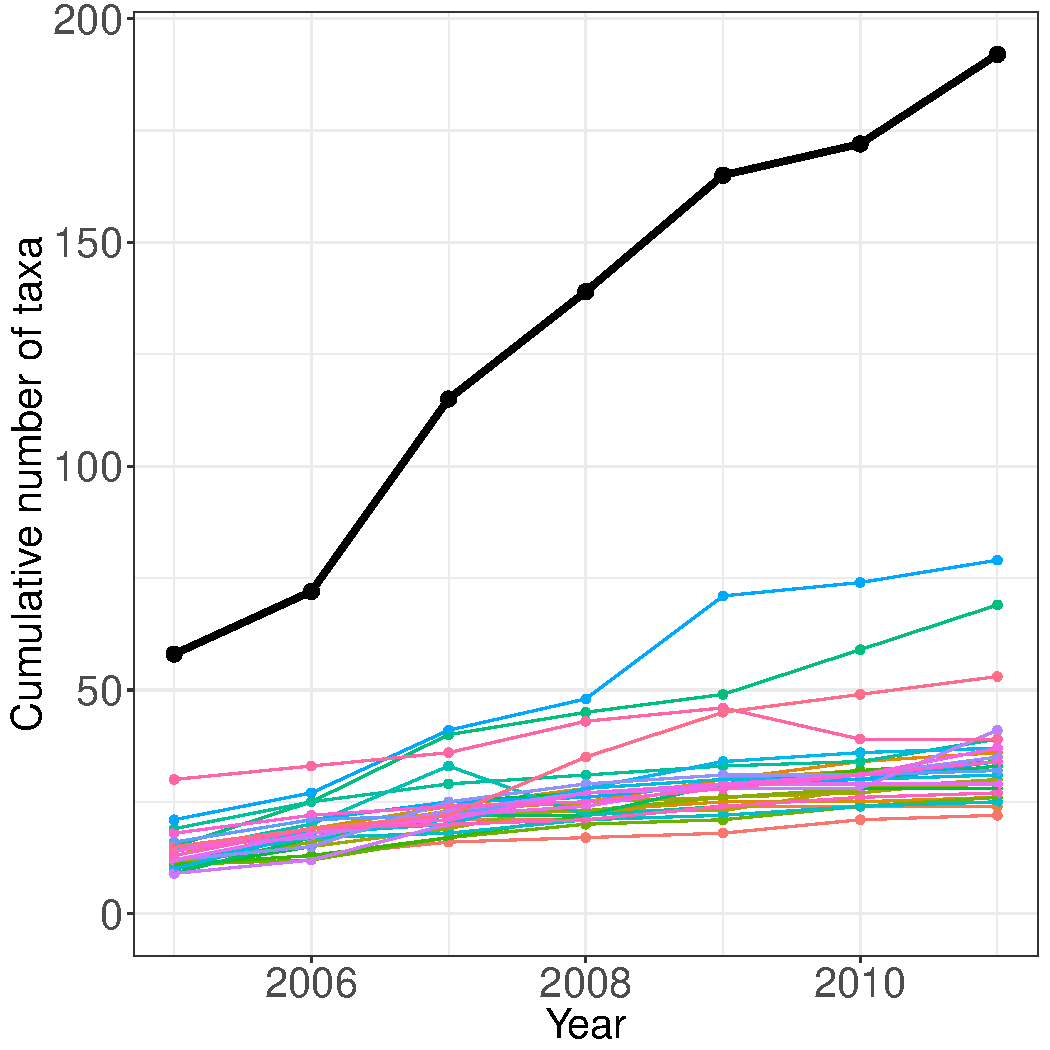
\includegraphics[scale = 0.4]{fce-diatoms-catano_species_accumulation_curve.pdf}
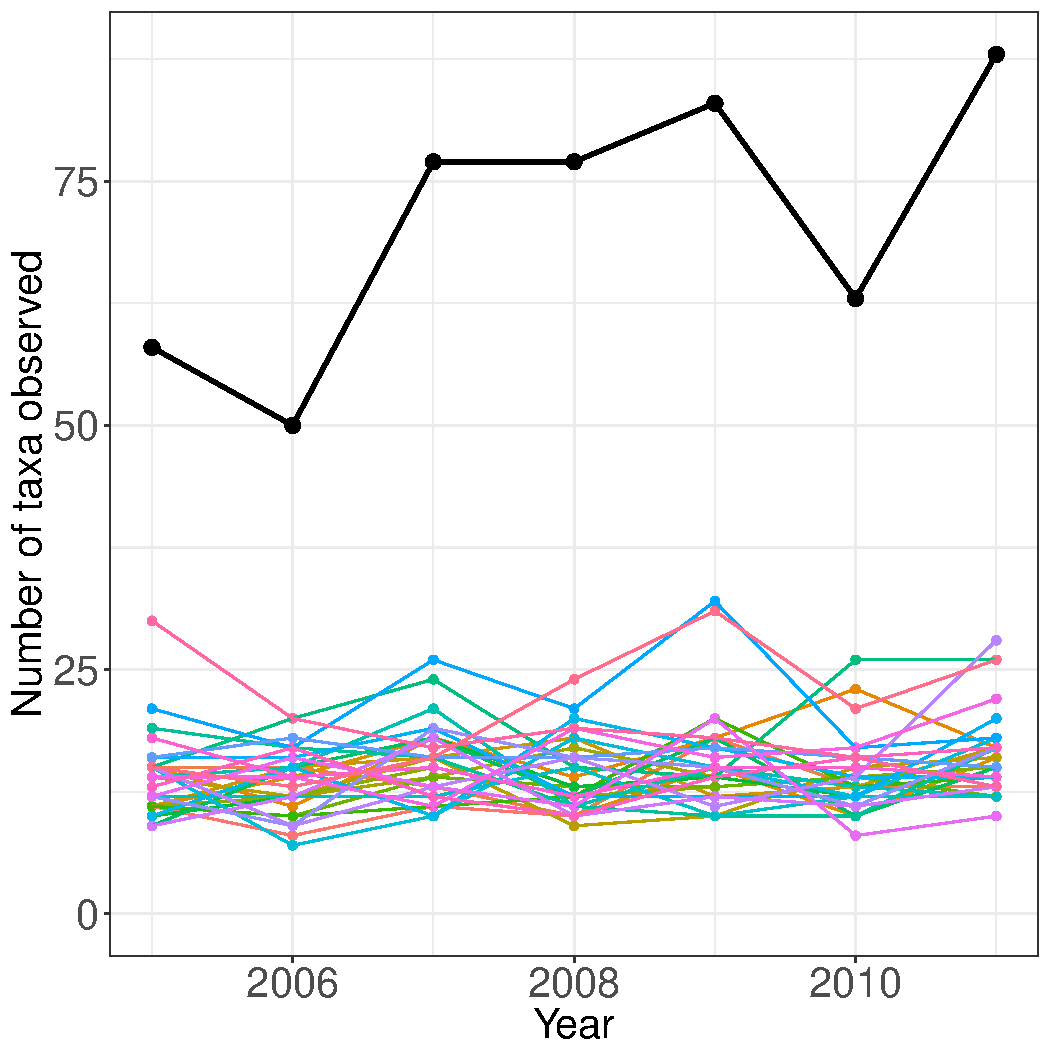
\includegraphics[scale = 0.4]{fce-diatoms-catano_num_taxa_over_time.pdf}
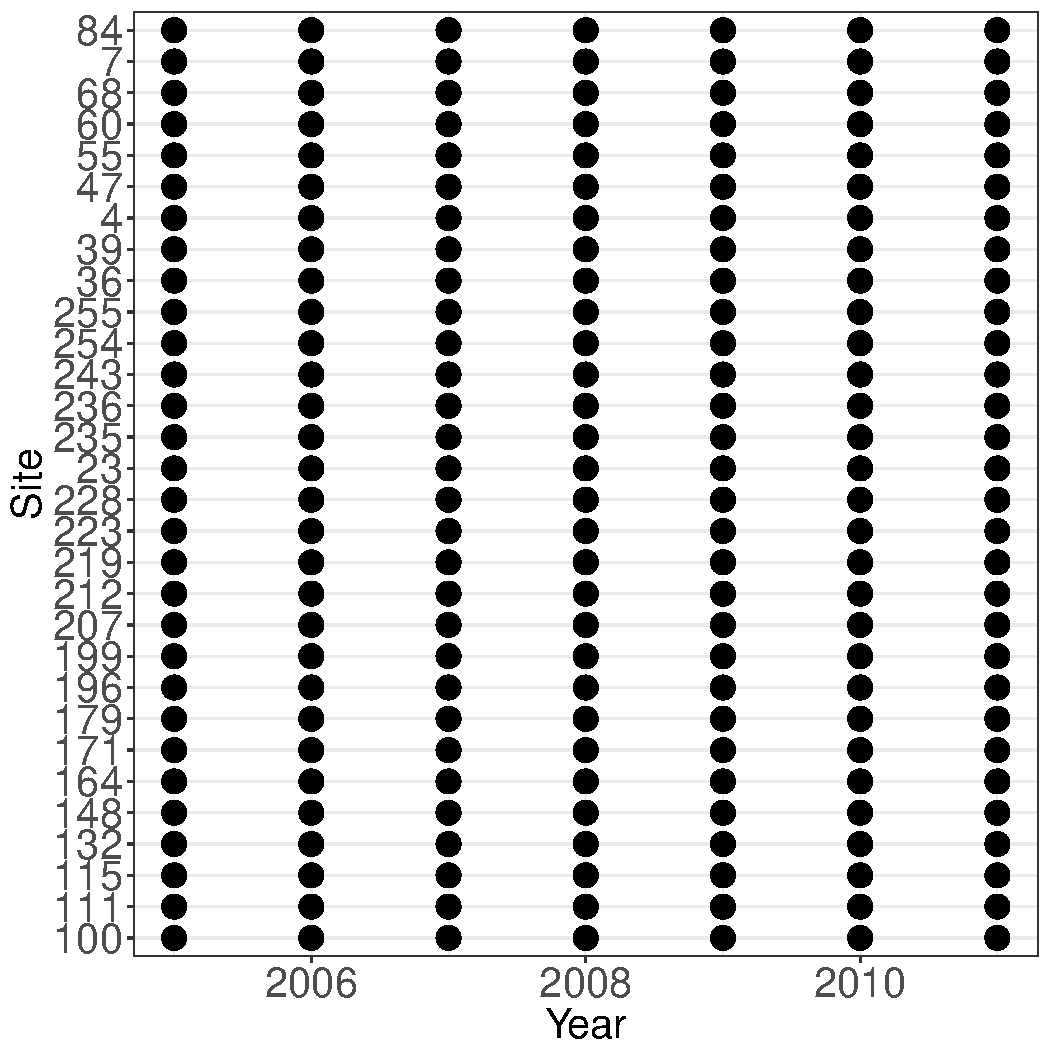
\includegraphics[scale = 0.4]{fce-diatoms-catano_spatiotemporal_sampling_effort.pdf}
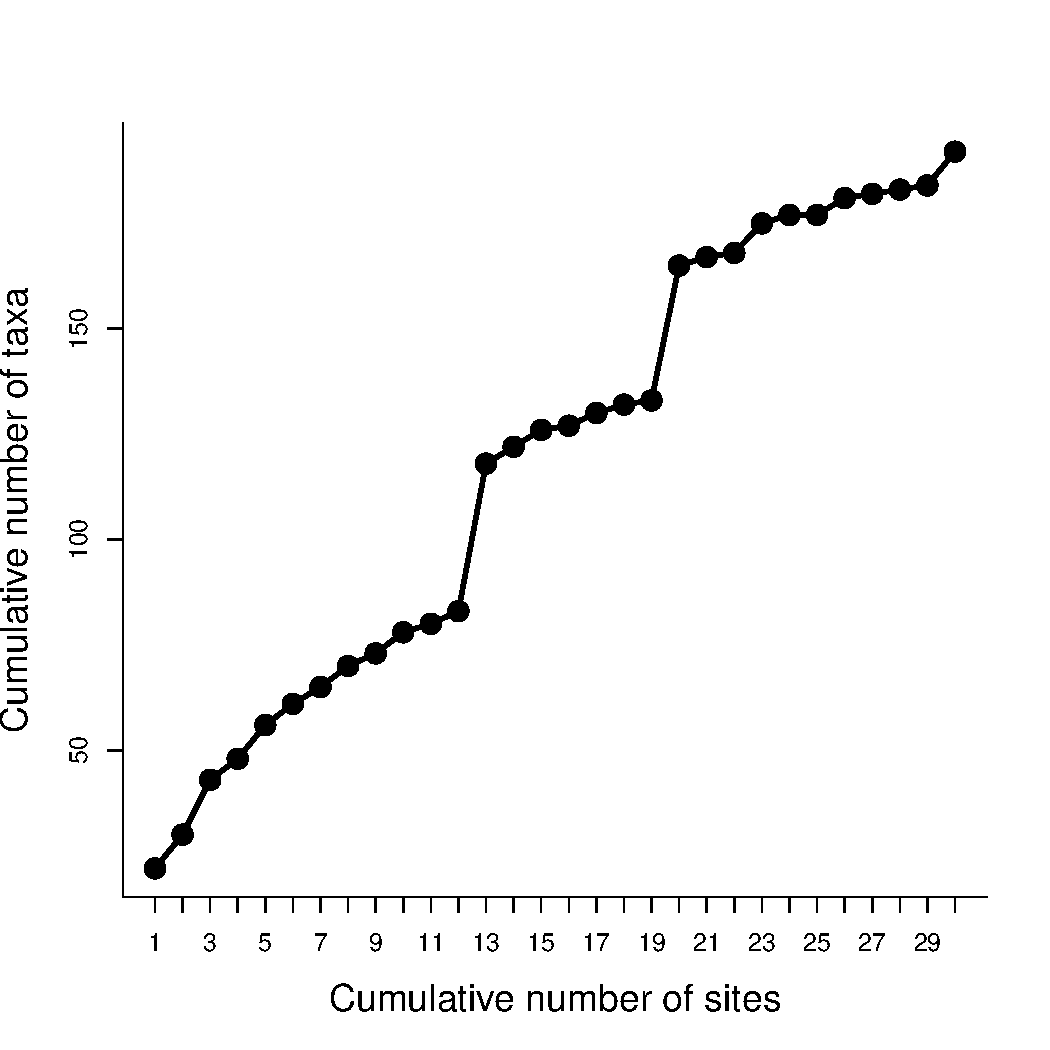
\includegraphics[scale = 0.4]{fce-diatoms-catano_species_accumulation_space.pdf}
\caption{{\bf FCE-diatoms:} Species accumulation curves (top left),  annual richness (top right), and sampling effort (bottom)  for diatom taxa observed at  Florida Coastal Everglades LTER. The black lines represent total site-level values across all plots.}
\label{fce-diatoms}
\end{figure}

\subsection {fce-fish}
{\bf Need to select wet or dry season.}
Data were obtained from the PI, and are cataloged on EDI  \citep{fce-fish}.
Catch per unit effort (CPUE) was calculated as (count/distance)*100
For each species, the CPUE was aggregated by summing the CPUE measured in each bout (i.e., replicate) within each Creek Number | River | YEAR | Season combination.
The format was re-arranged to reflect the aggregated CPUE (?total CPUE?) per season as columns and mean CPUE column was created by averaging the CPUE across the three seasons.
NOTE: After the first preliminary examination of the aggregated CPUE values the mean CPUE was ignored due to the unbalanced observations across the years and seasons. 
So, only the observations in the Wet and Dry season were considered.
Dry season: In this set, only the sites within RB were considered to create a balanced design for the analysis. 
Thus, this set encompassed a longer temporal range with a cost of less spatial replication.
NOTE: Also, YEAR 2004-2005 and 2011 were eliminated due to incomplete representation across the sites
Wet season: In this set both RB and TB were considered but only after 2010. Thus, this set has a wider spatial replication but a shorter temporal range.
NOTE: The difference in the spatial replication between seasons is related to the limitation of the sampling approach (electrofishing) which is limited to low salinity conditions. 
Salinity threshold for electrofishing is often reached in TB during the Dry season (i.e., TB is considered the estuarine portion of the Shark River System).
Data from the dry season are shown in Figure \ref{fce-fish-dry}.
Data from the wet season are shown in Figure \ref{fce-fish-wet}.

\begin{figure}[h!]
\centering
\includegraphics[scale = 0.4]{fce-fish-RehageDry_species_accumulation_curve.pdf}
\includegraphics[scale = 0.4]{fce-fish-RehageDry_num_taxa_over_time.pdf}
\includegraphics[scale = 0.4]{fce-fish-RehageDry_spatiotemporal_sampling_effort.pdf}
%\includegraphics[scale = 0.4]{fce-fish-RehageDry_spp_shared.pdf}
\caption{{\bf FCE-fish dry season:} Species accumulation curves (top left),  annual richness (top right), and sampling effort (bottom)  for fish taxa observed at the Florida Coastal Everglades . The black lines represent total site-level values across all plots.}
\label{fce-fish-dry}
\end{figure}

\begin{figure}[h!]
\centering
\includegraphics[scale = 0.4]{fce-fish-RehageWet_species_accumulation_curve.pdf}
\includegraphics[scale = 0.4]{fce-fish-RehageWet_num_taxa_over_time.pdf}
\includegraphics[scale = 0.4]{fce-fish-RehageWet_spatiotemporal_sampling_effort.pdf}
%\includegraphics[scale = 0.4]{fce-fish-RehageWet_spp_shared.pdf}
\caption{{\bf FCE-fish wet season:} Species accumulation curves (top left),  annual richness (top right), and sampling effort (bottom)  for fish taxa observed at the Florida Coastal Everglades . The black lines represent total site-level values across all plots.}
\label{fce-fish-wet}
\end{figure}



\newpage
\subsection {ntl-zooplankton}
The data were downloaded from the EDI Data Portal \citep{ntl-zooplankton}.
Samples were taken  via vertical tows at fortnightly intervals on a minimum of five occasions per year (range = 5 - 18 occasions per year).
Density was recorded as number of individuals per liter for each taxa, integrated volumetrically over the water column.
Many taxa are identified to species level, but some are identified to genus level.
Lake `Tr'  was only sampled in one year and was assumed to be the same as lake `TR'. %; thus we changed the lake identification code. 
The initial year (1981) was removed from analysis because only five of the seven lakes were sampled.
We additionally removed 165 records with missing or unknown taxa designations.
Data were aggregated annually for each taxa in each lake by taking the maximum density observed in a tow sampling occasion.
Data are shown in Figure \ref{ntl-zooplankton}.

\begin{figure}[h!]
\centering
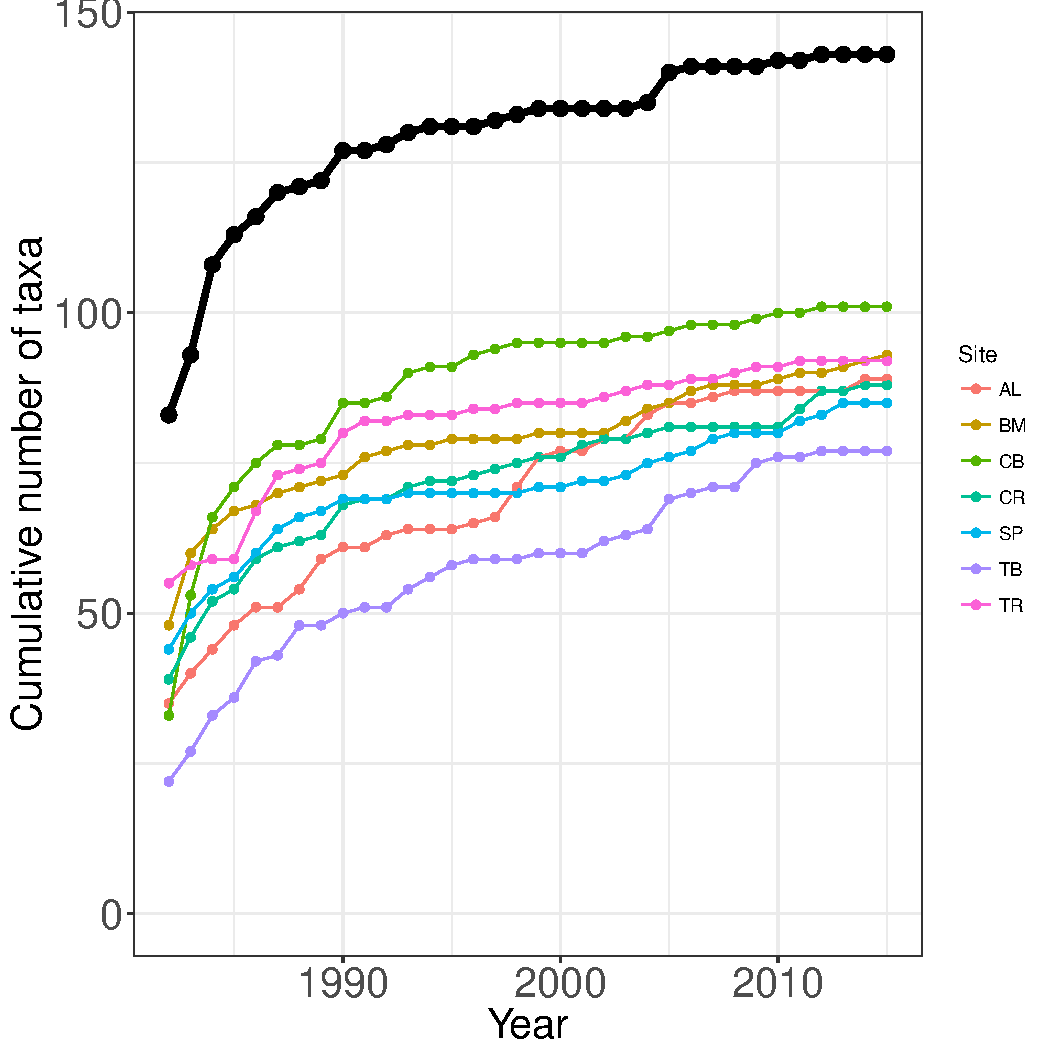
\includegraphics[scale = 0.4]{ntl-zooplankton-stanleyLottig_species_accumulation_curve.pdf}
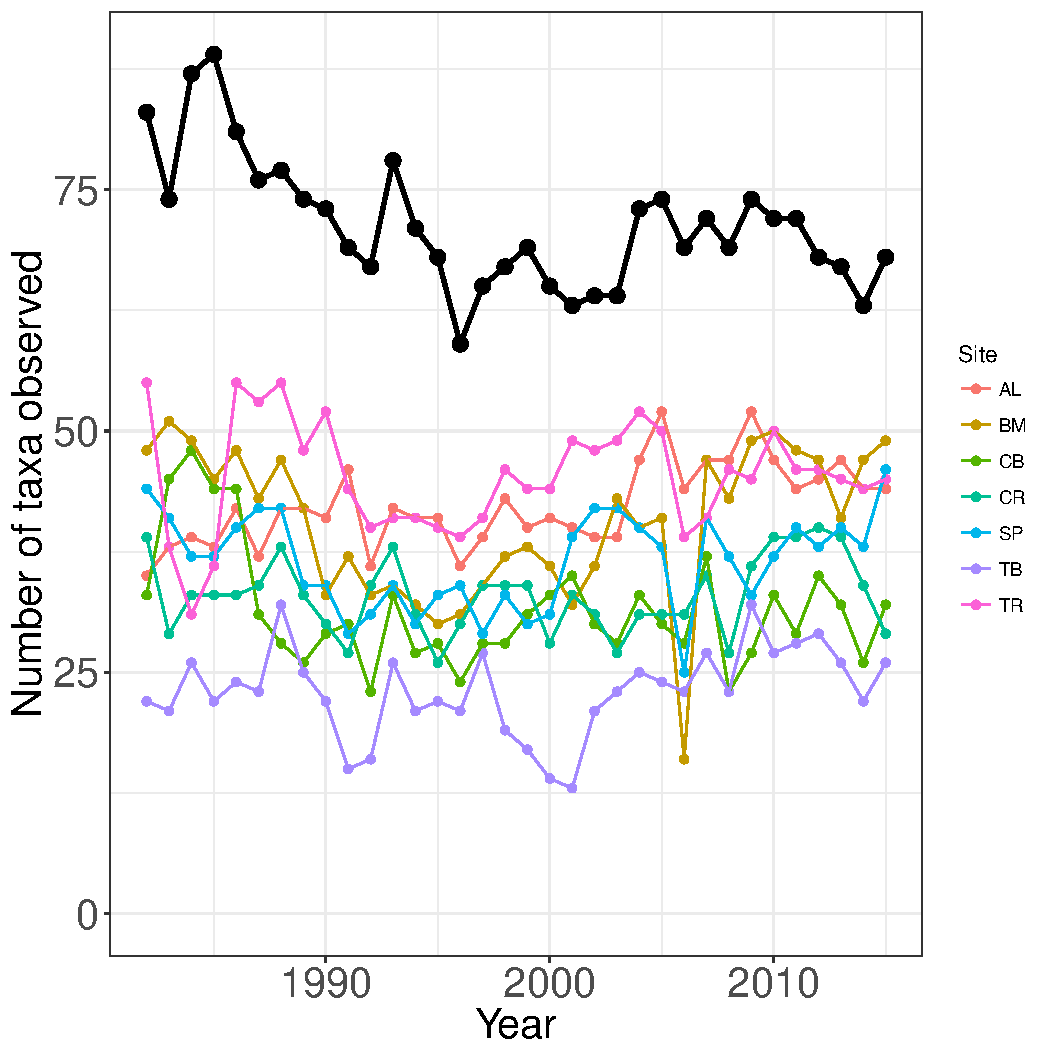
\includegraphics[scale = 0.4]{ntl-zooplankton-stanleyLottig_num_taxa_over_time.pdf}
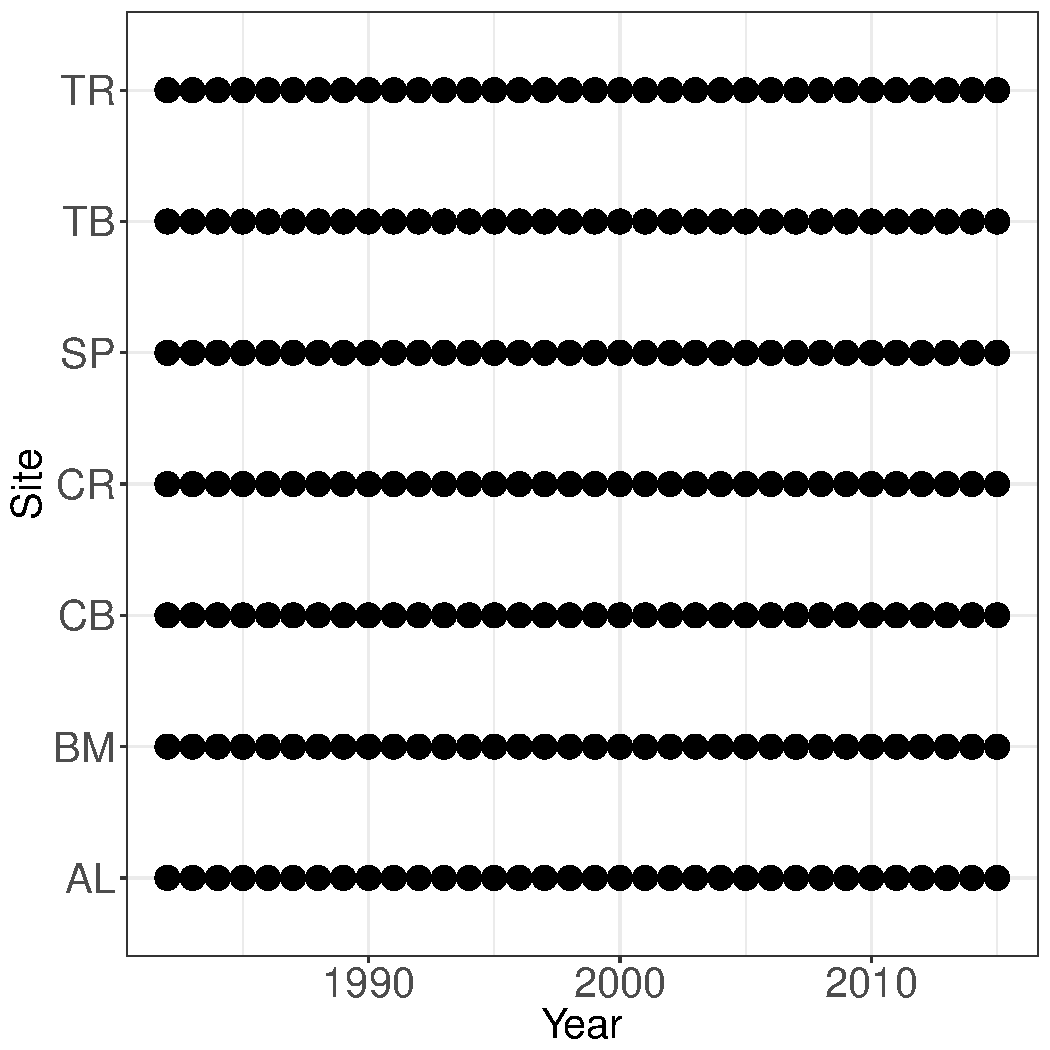
\includegraphics[scale = 0.4]{ntl-zooplankton-stanleyLottig_spatiotemporal_sampling_effort.pdf}
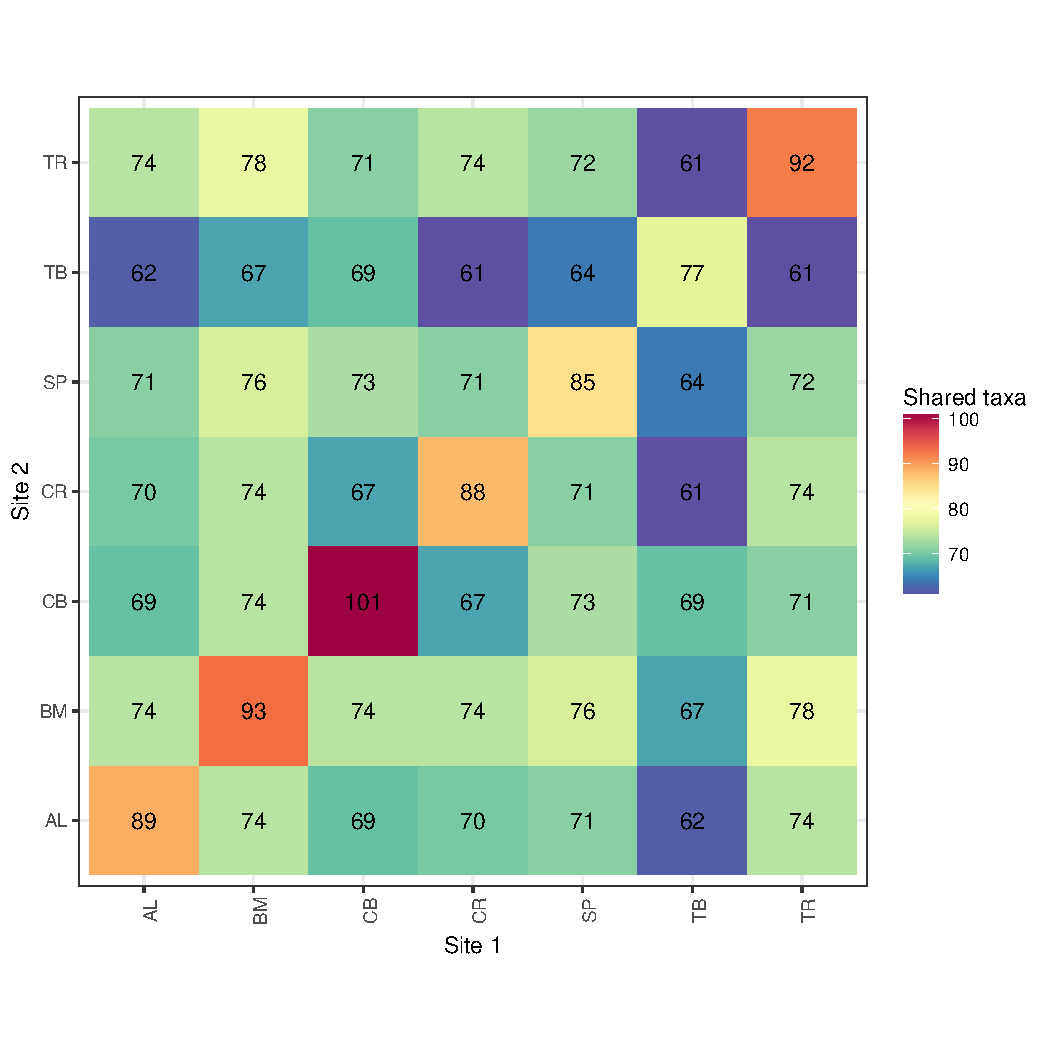
\includegraphics[scale = 0.4]{ntl-zooplankton-stanleyLottig_spp_shared.pdf}
\caption{{\bf NTL-zooplankton:} Species accumulation curves (top left),  annual richness (top right), and sampling effort (bottom)  for 143 zooplankton taxa observed at 7 sites North Temperate Lakes LTER . The black lines represent total site-level values across all plots. The plot of the species accumulation curve failed because one site was sampled in only one year, and will be fixed once that site is removed.}
\label{ntl-zooplankton}
\end{figure}


\subsection {ntl-fish}
{\bf species codes from the southern lakes were not dropped, so the metadata indicates there are 81 total species even though there are under 60.}
Data on fish abundance were downloaded from the EDI Data Portal \citep{ntl-fish}.
Two types of gill nets (VGN and VGN127) and the method  ``ESHOCK" were rarely used, and thus removed from the dataset.% as per a conversation with Noah Lottig at NTL.
The gear method ``ESHOCK" was also rarely used and a follow up call is needed to determine how best to handle those data.
They are currently included.
Catch per unit effort (CPUE) was calculated for each species in each lake per year across all gear types (electrofishing, gill nets, baited traps) as the total catch divided by the total effort.
We should double check with dataset contacts to be sure we did this correctly.
88 rows containing unidentified species were removed.
Also, the two bog lakes (CB, TB) had 1-3 species each and were removed. 
Only data from the northern lakes were included.
Data are shown in Figure \ref{ntl-fish}.

\begin{figure}[h!]
\centering
\includegraphics[scale = 0.4]{ntl-fish-stanleyLottig_species_accumulation_curve.pdf}
\includegraphics[scale = 0.4]{ntl-fish-stanleyLottig_num_taxa_over_time.pdf}
\includegraphics[scale = 0.4]{ntl-fish-stanleyLottig_spatiotemporal_sampling_effort.pdf}
\includegraphics[scale = 0.4]{ntl-fish-stanleyLottig_species_accumulation_space.pdf}
\includegraphics[scale = 0.4]{ntl-fish-stanleyLottig_spp_shared.pdf}
\caption{{\bf NTL-fish:} Species accumulation curves (top left),  annual richness (top right), and sampling effort (bottom)  for 81 fish species observed at 9 lakes in the North Temperate Lakes LTER (1995-2016). The black lines represent total site-level values across all plots.}
\label{ntl-fish}
\end{figure}


%%%%%%%%%%%%%%%%%%%
\section {Terrestrial datasets}


\subsection {and-plants-mtStHelens}
Data were downloaded from Ecological Archives \citep{and-plants} and are described in \citep{delMoral2005}..
We used data from the Pumice Plains habitat, which is the longest continuous sampling (about 20 years) for this dataset (Figure \ref{and-plants}).

\begin{figure}[h!]
\centering
\includegraphics[scale = 0.4]{and-plants-mtStHelens_species_accumulation_curve.pdf}
\includegraphics[scale = 0.4]{and-plants-mtStHelens_num_taxa_over_time.pdf}
\includegraphics[scale = 0.4]{and-plants-mtStHelens_spatiotemporal_sampling_effort.pdf}
\includegraphics[scale = 0.4]{and-plants-mtStHelens_spp_shared.pdf}
\caption{{\bf AND-plants:} Species accumulation curves (top left),  annual richness (top right), and sampling effort (bottom)  for plant species observed at Mt. St. Helens. The black lines represent total site-level values across all plots.}
\label{and-plants}
\end{figure}


\subsection {cdr-plants}
Data were downloaded from EDI \citep{cdr-plants}.
Annual censuses for dataset are incomplete after 2004, so we only consider data until 2004. 
We used data from control plots only, from all four sites (A, B, C, and D). 
Fields A, B, and C were considered together as a single dataset, while D was considered a separate datasets because of its unique fire history.
We cleaned taxonomic data by cleaning clear mistakes (such as `carex sp.' instead of `Carex sp.'), removed non-taxonomic entities (``Miscellaneous litter") and non-plant taxa (`Fungi', and `Mosses \& lichens').
We also lumped or dropped certain taxonomic information. 
In particular, we lumped taxonomic information to the genus level when more than 1$\%$ (more than a proportion of 0.01) of the biomass of a genus was not identified to the species level. 
For example, {\it Cyperus} species are usually identified to the genus level (``Cyperus  sp.") rather than species level (``{\it Cyperus schweinitzii}''), with a minority of the biomass (less than 10$\%$) identified at the specific level. We therefore consider only genus information for {\it Cyperus}. 
We dropped taxonomic information when within a certain genus, biomass is identified to the genus level. 
For example, in the genus {\it Viola}, more than 99.8$\%$ of biomass was determined to the species level. We therefore dropped from the dataset the instances when biomass is assigned to 'Viola sp.'.
Data are shown in figures \ref{cdr-plantsABC} and \ref{cdr-plantsD}.

\begin{figure}[h!]
\centering
\includegraphics[scale = 0.4]{cdr-plantsABC-compagnoni_species_accumulation_curve.pdf}
\includegraphics[scale = 0.4]{cdr-plantsABC-compagnoni_num_taxa_over_time.pdf}
\includegraphics[scale = 0.4]{cdr-plantsABC-compagnoni_spatiotemporal_sampling_effort.pdf}
\includegraphics[scale = 0.4]{cdr-plantsABC-compagnoni_species_accumulation_space.pdf}
\includegraphics[scale = 0.4]{cdr-plantsABC-compagnoni_spp_shared.pdf}
\caption{{\bf CDR-plants, A, B, and C fields:} Species accumulation curves (top left),  annual richness (top right), and sampling effort (bottom)  for plant species observed in the A, B, and C fields at Cedar Creek. The black lines represent total site-level values across all plots.}
\label{cdrABC-plants}
\end{figure}


\begin{figure}[h!]
\centering
\includegraphics[scale = 0.4]{cdr-plantsD-compagnoni_species_accumulation_curve.pdf}
\includegraphics[scale = 0.4]{cdr-plantsD-compagnoni_num_taxa_over_time.pdf}
\includegraphics[scale = 0.4]{cdr-plantsD-compagnoni_spatiotemporal_sampling_effort.pdf}
\includegraphics[scale = 0.4]{cdr-plantsD-compagnoni_species_accumulation_space.pdf}
\includegraphics[scale = 0.4]{cdr-plantsD-compagnoni_spp_shared.pdf}
\caption{{\bf CDR-plants, D field:} Species accumulation curves (top left),  annual richness (top right), and sampling effort (bottom)  for plant species observed in the D field at Cedar Creek. The black lines represent total site-level values across all plots.}
\label{cdrD-plants}
\end{figure}


\subsection{sgs-plants}
Data were downloaded from EDI \citep{sgs-plants}.
Plant community composition on the three grassland and three shrubland small mammal trapping webs (hereafter called ?sites?; n = 6). 
Vegetation measurements were made once per year, usually in mid-July. 
Percent canopy cover of each plant species was estimated visually in 30 0.10-m2 Daubenmire quadrats on each web. 
We aggregated plant species percent cover data at the ?site? scale because each year, transects and plot locations were determined based on a randomization procedure (3 trap stations were chosen randomly within each site from a list of 12 permanent points, where transects with random orientations were centered on each trap station location). 
Trapping web ?31W? was removed because it was sampled in only 2 years (2006 and 2007).
Samples for year 2007 were removed because not all sites were sampled in 2007.
Species codes that did not identify plant species were removed (litter, bare ground, etc.).
Species codes that were otherwise inconsistent (different cases, naming conventions, etc.) were reconciled so that all species were identified by unique 4 letter codes.
Observations for codes that did not represent plants, or plants were unknown or not resolved to species were removed prior to analysis.
Data are shown in Figure \ref{sgs-plants}.
\begin{figure}[h!]
\centering
\includegraphics[scale = 0.4]{sgs-plants-catano_species_accumulation_curve.pdf}
\includegraphics[scale = 0.4]{sgs-plants-catano_num_taxa_over_time.pdf}
\includegraphics[scale = 0.4]{sgs-plants-catano_spatiotemporal_sampling_effort.pdf}
\includegraphics[scale = 0.4]{sgs-plants-catano_species_accumulation_space.pdf}
\includegraphics[scale = 0.4]{sgs-plants-catano_spp_shared.pdf}
\caption{{\bf SGS-plants:} Species accumulation curves (top left),  annual richness (top right), and sampling effort (bottom)  for plant species observed at the Shortgrass Steppe (SGS) LTER. The black lines represent total site-level values across all plots.}
\label{sgs-plants}
\end{figure}

\subsection{jrn-plants}
We selected a subsample of 10 quadrats that provided 18 sampling occasions over 24 years (1915-1938). 
This is a small subsample of the 114 quadrats that make up this incredible dataset. 
We then dropped or lumped taxonomic identifiers, because several counts were assigned to a genus rather than to a species. 
For 25 genera contained in this dataset, counts were sometimes assigned to a species (e.g. Poa secunda) or to a genus (e.g. Poa spp.). 
In such cases, we calculated the total proportion (within the entire dataset) of counts assigned to a genus level. 
When the percentage of counts identified to a genus were less than 5$\%$ of the total counts, we discarded the information. 
However, when the the percentage of counts identified at the genus level was more than 5$\%$, we lumped all of the counts assigned to a species into a single genus. 
We did this because such high proportion of counts assigned to a genus, rather than a species, suggests high uncertainty in species identification.
NOTE: the species accumulation curve in this dataset saturated quite rapidly. This is potentially an artifact of "lumping" specific information to the genus level. 
Data are shown in Figure \ref{jrn-plants}.

\begin{figure}[h!]
\centering
\includegraphics[scale = 0.4]{jrn-plants-compagnoni_species_accumulation_curve.pdf}
\includegraphics[scale = 0.4]{jrn-plants-compagnoni_num_taxa_over_time.pdf}
\includegraphics[scale = 0.4]{jrn-plants-compagnoni_spatiotemporal_sampling_effort.pdf}
\includegraphics[scale = 0.4]{jrn-plants-compagnoni_species_accumulation_space.pdf}
\includegraphics[scale = 0.4]{jrn-plants-compagnoni_spp_shared.pdf}
\caption{{\bf JRN-plants:} Species accumulation curves (top left),  annual richness (top right), and sampling effort (bottom)  for plant species observed at the Jornada (JRN) LTER. The black lines represent total site-level values across all plots.}
\label{jrn-plants}
\end{figure}


\subsection {sev-grasshoppers}
The data were downloaded from the EDI Data Portal \citep{sev-grasshopper}.
We retained data from only two habitats (Black grama and Creosotebush) that shared many species, and presented 20 years of temporal replication. This data were collected twice a year, and spatial replication included site, transect, and web. 
Population (count) data is structured, being collected across sex, age, and substrate. 
We summed numbers across webs, sex, age, and substrate.
Data are shown in Figure \ref{sev-grasshoppers}.
  

\begin{figure}[h!]
\centering
\includegraphics[scale = 0.4]{sev-grasshopper-compagnoni_species_accumulation_curve.pdf}
\includegraphics[scale = 0.4]{sev-grasshopper-compagnoni_num_taxa_over_time.pdf}
\includegraphics[scale = 0.4]{sev-grasshopper-compagnoni_spatiotemporal_sampling_effort.pdf}
\includegraphics[scale = 0.4]{sev-grasshopper-compagnoni_spp_shared.pdf}
\caption{{\bf SEV-grasshoppers:} Species accumulation curves (top left),  annual richness (top right), spatio-temporal sampling effort (bottom left), and number of shared species (bottom right) for grasshopper species observed in Black grama (BOER) and Creosotebush (LATR) habitats the Sevilleta LTER (1992-2013). The black lines represent total site-level values across all plots.}
\label{sev-grasshoppers}
\end{figure}


\subsection{cdr-grasshoppers}
Data were accessed on EDI \citep{cdr-grasshoppers}.
We removed sites `28' and `11', which were added to the sampling after 1989. 
Then, we summed the number of individuals across all life stages and all months. 
We summed across months even if in 2003, June and August samples were lost for some fields. 
However, as the documentation reports, ``The total counts for these fields were augmented by proportional additions from remaining samples by John Haarstad and crew".
Taxonomic information is available for only for the {\it Acrididae} family before 1994. 
We lumped taxonomic identifications to genus level for {\it Conocephalus}, {\it Scudderia}, and {it\ Tetrix}, as too high a proportion of individuals from these genera were not identified at the species level. 
Similarly, some individuals belonging to the {\it Melanoplus} genus were identified at the genus level only. 
We removed these records, as they comprised only 6$\%$ of the entire counts in the {\it Melanoplus} genus.
Data are shown in Figure \ref{cdr-grasshoppers}.

\begin{figure}[h!]
\centering
\includegraphics[scale = 0.4]{cdr-grasshopper-compagnoni_species_accumulation_curve.pdf}
\includegraphics[scale = 0.4]{cdr-grasshopper-compagnoni_num_taxa_over_time.pdf}
\includegraphics[scale = 0.4]{cdr-grasshopper-compagnoni_spatiotemporal_sampling_effort.pdf}
\includegraphics[scale = 0.4]{cdr-grasshopper-compagnoni_species_accumulation_space.pdf}
\includegraphics[scale = 0.4]{cdr-grasshopper-compagnoni_spp_shared.pdf}
\caption{{\bf CDR-grasshoppers:} Species accumulation curves (top left),  annual richness (top right), spatio-temporal sampling effort (bottom left), and number of shared species (bottom right) for grasshopper species observed at the Cedar Creek LTER. The black lines represent total site-level values across all plots.}
\label{cdr-grasshoppers}
\end{figure}



\subsection{knz-grasshoppers}
Data on grasshopper abundance (1996-2015) were downloaded from  EDI \citep{knz-grasshoppers}.
We retained 13 spatial replicates which provide continuous temporal replicates from 1995 to 2013 (2012 is missing). 
We lumped taxonomic information level whenever the counts at the genus level made up more than 5$\%$ of the total individuals counted. 
We did not do this lumping for {\it Melanopus} spp. because it is a hyperdiverse genus. 
In this case, we dropped all {\it Melanopus} records identified at the genus level. 
Finally, we average count data across a year, because some spatial replicates could occasionally contain more observations within a year.
Data are shown in Figure \ref{knz-grasshoppers}.


\begin{figure}[h!]
\centering
\includegraphics[scale = 0.4]{knz-grasshopper-compagnoni_species_accumulation_curve.pdf}
\includegraphics[scale = 0.4]{knz-grasshopper-compagnoni_num_taxa_over_time.pdf}
\includegraphics[scale = 0.4]{knz-grasshopper-compagnoni_spatiotemporal_sampling_effort.pdf}
%\includegraphics[scale = 0.4]{knz-grasshopper-compagnoni_spp_shared.pdf}
\includegraphics[scale = 0.4]{knz-grasshopper-compagnoni_species_accumulation_space.pdf}
\caption{{\bf KNZ-grasshoppers:} Species accumulation curves (top left),  annual richness (top right), spatio-temporal sampling effort (bottom left), and number of shared species (bottom right) for grasshopper species observed in ... The black lines represent total site-level values across all plots.}
\label{knz-grasshoppers}
\end{figure}

\subsection{luq-snails}
Data were downloaded from EDI \citep{luq-snails}.
We averaged number of snails across runs ("Run.ID" in dataset) and seasons ("Seasons" in dataset). 
There were no codes for unknown or non-living taxa.
Data are shown in Figure \ref{luq-snails}.

\begin{figure}[h!]
\centering
\includegraphics[scale = 0.4]{luq-snails-compagnoni_species_accumulation_curve.pdf}
\includegraphics[scale = 0.4]{luq-snails-compagnoni_num_taxa_over_time.pdf}
\includegraphics[scale = 0.4]{luq-snails-compagnoni_spatiotemporal_sampling_effort.pdf}
\includegraphics[scale = 0.4]{luq-snails-compagnoni_spp_shared.pdf}
\includegraphics[scale = 0.4]{luq-snails-compagnoni_species_accumulation_space.pdf}
\caption{{\bf LUQ-snails:} Species accumulation curves (top left),  annual richness (top right), spatio-temporal sampling effort (bottom left), and number of shared species (bottom right) for snail species observed in Luquillo LTER. The black lines represent total site-level values across all plots.}
\label{luq-snails}
\end{figure}


\subsection {jrn-lizards}
The data were downloaded from the EDI Data Portal \citep{jrn-lizard}.
This was a mark-recapture study. 
Pitfall traps were opened for two weeks four times per year (quarterly). 
The monthly samples from 1990 and 1991 were removed.
Individual lizards were identified and the number of unique individuals per site per year were summed. 
Two sites that were established five years after the start of the study (SUMM and NORT) were excluded. 
We don't have a key to the species codes.
Data are shown in Figure \ref{jrn-lizards}.
The cumulative number of taxa was still increasing at the end of the time series, although with only 20 species total one or two species introductions could cause this pattern.


\begin{figure}[h!]
\centering
\includegraphics[scale = 0.4]{jrn-lizards-hope_species_accumulation_curve.pdf}
\includegraphics[scale = 0.4]{jrn-lizards-hope_num_taxa_over_time.pdf}
\includegraphics[scale = 0.4]{jrn-lizards-hope_species_accumulation_space.pdf}
\includegraphics[scale = 0.4]{jrn-lizards-hope_spatiotemporal_sampling_effort.pdf}
\includegraphics[scale = 0.4]{jrn-lizards-hope_spp_shared.pdf}
\caption{{\bf JRN-lizards:} Species accumulation curves (top left),  annual richness (top right), and sampling effort (bottom)  for 20 lizard species observed at 9 plots in the Jornada LTER (1990-2005). The black lines represent total site-level values across all plots.}
\label{jrn-lizards}
\end{figure}



\subsection {cap-herps}
The data were downloaded from the EDI Data Portal \citep{cap-herps}.
Data are shown in Figure \ref{cap-herps}.
This is a visual encounter survey where herpetofauna observations were nested by 3 plots within 3 transects per site. 
Each site represents the reach level (each reach level site is composed of 3 transects with equal area sampling efforts). 
Surveys from 2012 and March were dropped to standardize sampling efforts temporally. 
Unidentified species were dropped, species code is the scientific name of species. 
Taxon count was calculated as the maximum abundance per year in any one of the sampling events (with 3 sampling events per reach in April/May, June/July, and September/October). 
The final community dataset prepared for analysis has 7 sites representative of the reach level metacommunity dynamics (3 transects sampled per reach) from 2013-2017 with a total of 18 observed species across all sites.  

\begin{figure}[h!]
\centering
\includegraphics[scale = 0.4]{cap-herps-banville_species_accumulation_curve.pdf}
\includegraphics[scale = 0.4]{cap-herps-banville_num_taxa_over_time.pdf}
\includegraphics[scale = 0.4]{cap-herps-banville_spatiotemporal_sampling_effort.pdf}
\includegraphics[scale = 0.4]{cap-herps-banville_spp_shared.pdf}
\caption{{\bf CAP-herps:} Species accumulation curves (top left),  annual richness (top right), and sampling effort (bottom)  for species observed in the Central Area Phoenix LTER (1990-2005). The black lines represent total site-level values across all plots.}
\label{cap-herps}
\end{figure}


\subsection {and-birds}
The data were downloaded from the EDI Data Portal \citep{and-birds}.
We used data from the first five years of study (2009 - 2013) because six counts per season were conducted in those years.
We summed the counts of new individuals observed within the closest distance radius (> 50 m)  of the points during the 10-minute interval for on each sampling occasion, and used the maximum number of individuals of each species recorded at each point as the abundance value for that year.
Data are shown in Figure \ref{and-birds}.

\begin{figure}[h!]
\centering
\includegraphics[scale = 0.4]{and-birds-wisnoski_species_accumulation_curve.pdf}
\includegraphics[scale = 0.4]{and-birds-wisnoski_num_taxa_over_time.pdf}
\includegraphics[scale = 0.4]{and-birds-wisnoski_spatiotemporal_sampling_effort.pdf}
%\includegraphics[scale = 0.4]{and-birds-wisnoski_spp_shared.pdf}
\caption{{\bf AND-birds:} }
\label{and-birds}
\end{figure}


\subsection {hbr-birds}
{\bf Need to subset by date so only 1-2 sampling occasions per year are included.}
These point count data were downloaded from the EDI Data Portal \citep{hbr-birds}.
Years with highly incomplete sampling were removed (1999, 2000, 2008) and only plots that were sampled in all of the remaining years were retained for analysis.
The number of individuals of each species within 50 m of the `point' was summed for each 10-minute plot visit, using the `NewRecord' column to identify unique individuals for data collected after 2005. 
The maximum number of individuals of each species for each plot-year (across 1-3 sampling occasions in June/early July per year)  was calculated.
Data are shown in Figure \ref{hbr-birds}.


\begin{figure}[h!]
\centering
\includegraphics[scale = 0.4]{hbr-birds-sillett_species_accumulation_curve.pdf}
\includegraphics[scale = 0.4]{hbr-birds-sillett_num_taxa_over_time.pdf}
\includegraphics[scale = 0.4]{hbr-birds-sillett_spatiotemporal_sampling_effort.pdf}
\includegraphics[scale = 0.4]{hbr-birds-sillett_spp_shared.pdf}
\caption{{\bf HBR-birds:} }
\label{hbr-birds}
\end{figure}

\subsection{cap-birds}
Data were obtained from EDI \citep{cap-birds}.
Data are shown in Figure \ref{cap-birds}.
This is a point count study where birds were observed (seen or heard) for 15 minutes within a 40 m fixed radius. 
Each site represents one point count. 
Only ESCA point counts are included. 
Data from 2017 were dropped because not all sites were sampled. 
Four point count sites (M-9, V-18, X-8, and V-16) were dropped due to uneven sampling across years. 
Unidentified species accounted for less then 2\% of the total data and were dropped. 
%Species codes are 4-letter codes (https://www.wintuaudubon.org/Documents/Alpha_codes_eng.pdf). 
Taxon count was calculated as the maximum abundance per year during the spring month's sampling events (with 3 sampling events per site between March, April, and May). 
  

\begin{figure}[h!]
\centering
\includegraphics[scale = 0.4]{cap-birds-banville_species_accumulation_curve.pdf}
\includegraphics[scale = 0.4]{cap-birds-banville_num_taxa_over_time.pdf}
\includegraphics[scale = 0.4]{cap-birds-banville_spatiotemporal_sampling_effort.pdf}
\includegraphics[scale = 0.4]{cap-birds-banville_spp_shared.pdf}
\caption{{\bf CAP-birds:} }
\label{cap-birds}
\end{figure}

\subsection{bes-birds}
Data were downloaded from EDI \citep{bes-birds}. We dropped all observations in the distance catagory ``FT" and all observations not identified to species. 
We only used sites with surveys every year from 2005-2009. 
When there was multiple surveys per year for a single site, the abundance counts were aggregated to the maximum observed count from any survey for each species at the respective site.
We only included plots in which at least one bird was observed in each year of study.
Data are shown in (Figure \ref{bes-birds}).
\begin{figure}[h!]
\centering
\includegraphics[scale = 0.4]{bes-birds-nilon_species_accumulation_curve.pdf}
\includegraphics[scale = 0.4]{bes-birds-nilon_num_taxa_over_time.pdf}
\includegraphics[scale = 0.4]{bes-birds-nilon_spatiotemporal_sampling_effort.pdf}
\includegraphics[scale = 0.4]{bes-birds-nilon_species_accumulation_space.pdf}
\includegraphics[scale = 0.4]{bes-birds-nilon_spp_shared.pdf}
\caption{{\bf BES-birds:} }
\label{bes-birds}
\end{figure}


\bibliographystyle{apalike}
\renewcommand{\refname}{\subsection*{References}}
\bibliography{LTER_metacom}

\end{document}
